\documentclass[conference]{IEEEtran}
\IEEEoverridecommandlockouts

% Core packages
\usepackage{cite}
\usepackage[T1]{fontenc}
\usepackage{hyperref}

% Math packages
\usepackage{amsmath,amssymb,amsfonts}
\usepackage{array,booktabs}

% Graphics and layout
\usepackage{graphicx}
\usepackage{subcaption}
\usepackage{float}
\usepackage{multirow}
\usepackage{multicol}
\usepackage{balance}

% Algorithm and code
\usepackage{algorithm}
\usepackage{algpseudocode} 
\usepackage{algorithmicx}
\usepackage{listings}

% Text and formatting
\usepackage{textcomp}
\usepackage{url}
\usepackage{enumitem}
\usepackage{caption} 
\usepackage{tcolorbox}

\usepackage[ngerman,main=english]{babel}

% TikZ for diagrams
\usepackage{tikz}
\usetikzlibrary{arrows.meta,shapes,positioning}
\usetikzlibrary{calc,angles,quotes}

% --- Macro for drawing a 2D spherocylinder ---
% #1 = center coordinate
% #2 = rotation angle
% #3 = half-length
% #4 = radius
\newcommand{\drawSpherocyl}[4]{
    \begin{scope}[shift={(#1)},rotate=#2]
        \draw[line width=1pt,rounded corners=6pt] (-#3,#4) -- (#3,#4);
        \draw[line width=1pt,rounded corners=6pt] (-#3,-#4) -- (#3,-#4);
        \draw[line width=1pt,rounded corners=6pt] (#3,-#4) arc[start angle=-90,end angle=90,radius=#4];
        \draw[line width=1pt,rounded corners=6pt] (-#3,#4) arc[start angle=90,end angle=270,radius=#4];
        \fill [black] (#1) circle (2pt);
    \end{scope}
}



\hypersetup{hidelinks}
\DeclareMathAlphabet\mathbfcal{OMS}{cmsy}{b}{n}

% Macro for growth comparison row
\newlength{\subfigwidth}
\setlength{\subfigwidth}{0.2\textwidth}
\newcolumntype{M}[1]{>{\centering\arraybackslash}m{#1}}

\newcommand{\growthcomparisonrow}[6]{%
    #1 &
    \begin{subfigure}[b]{\subfigwidth}
        \includegraphics[width=\textwidth]{figures/growth_comparison_lambda_#2/#1_#2.#3.jpeg}
    \end{subfigure} &
    \begin{subfigure}[b]{\subfigwidth}
        \includegraphics[width=\textwidth]{figures/growth_comparison_lambda_#2/#1_#2.#4.jpeg}
    \end{subfigure} &
    \begin{subfigure}[b]{\subfigwidth}
        \includegraphics[width=\textwidth]{figures/growth_comparison_lambda_#2/#1_#2.#5.jpeg}
    \end{subfigure} &
    \begin{subfigure}[b]{\subfigwidth}
        \includegraphics[width=\textwidth]{figures/growth_comparison_lambda_#2/#1_#2.#6.jpeg}
    \end{subfigure}  \\
}

\begin{document}

\title{Proliferating Cell Collectives: \\A Comparison of Hard and Soft Collision Models}

\author{
    \IEEEauthorblockN{Manuel Lerchner}
    \IEEEauthorblockA{
        \textit{Technical University of Munich}\\
        Munich, Germany}
}

\maketitle

\begin{abstract}
    This work investigates the computational modeling of proliferating cell collectives, comparing an established constraint-based collision model as developed by \cite{Weady2024} with a simpler potential-based collision model. While both approaches are demonstrated to reproduce key emergent patterns observed in bacterial colony growth, we highlight that ...............

\end{abstract}

\begin{IEEEkeywords}
    active matter, cell collectives, particle simulation, soft collision model, hard collision model, pattern formation, computational biology, performance comparison, agent-based modeling
\end{IEEEkeywords}

\section{Introduction}
\subsection{Biological Motivation}

The collective behaviors of biological entities, ranging from simple microbial colonies to complex multicellular tissues, are fundamental to unraveling the intricate processes of life. These systems often exhibit emergent spatio-temporal patterns, driven by the interplay of simple local interactions and individual growth dynamics. Bacterial colonies, for instance, showcase remarkable self-organization, developing sophisticated spatial structures in response to environmental stimuli. Specifically, experimental observations have highlighted the phenomenon of growth rate reduction in the colony's center due to mechanical pressure exerted by surrounding cells \cite{Wittmann2023}. For various bacteria, such as E. coli, Bacillus subtilis, and Proteus mirabilis, and fungi like Setosphaeria rostrata and Exserohilum Turcicum, which experience different local cell densities across their growth phases, this pressure-induced deceleration contributes to the formation of characteristic concentric ring patterns \cite{YAMAZAKI2005136}.

\begin{figure}
    \centering
    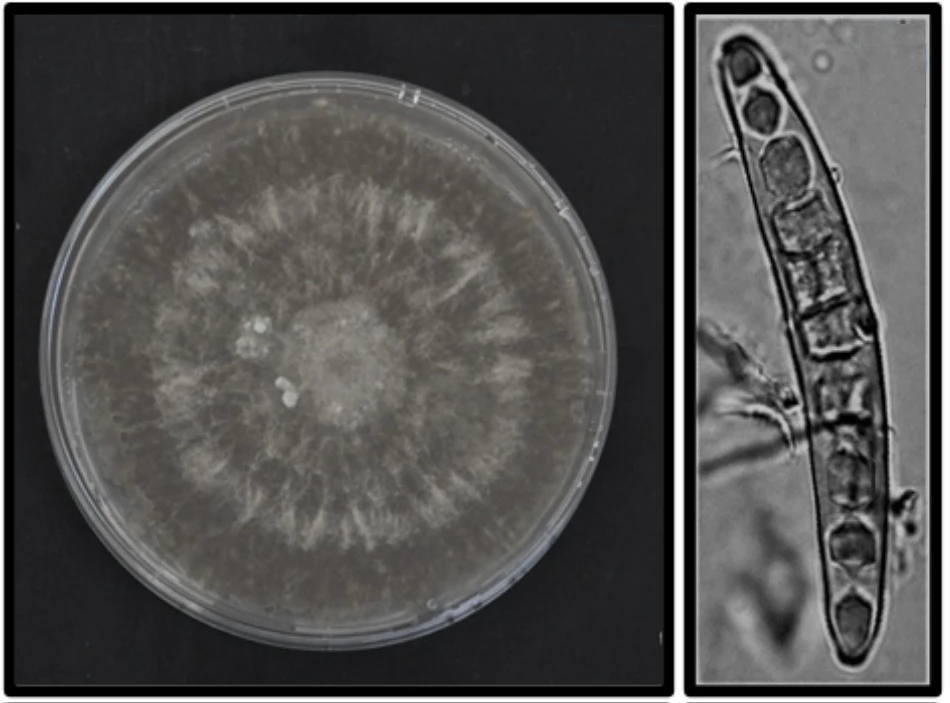
\includegraphics[width=\linewidth]{figures/real-bacteria/Exserohilum turcicum.png}
    \caption{Morphology of \textit{Exserohilum turcicum}. The left image displays a colony of Exserohilum turcicum, while the right image shows a single cell of the same species. Source: \cite{Bankole2023}.}
    \label{fig:exserohilum_turcicum}
\end{figure}

These biologically fascinating phenomena pose significant computational modeling challenges, demanding the accurate integration of both mechanical cell interactions and proliferation dynamics.

This work is directly inspired by these observations, particularly the formation of concentric rings in growing bacterial communities. These patterns represent a key manifestation of self-organization under controlled conditions, as further explored in \cite{Weady2024}. Comprehending these emergent structures necessitates robust computational models capable of capturing the dynamic interplay between individual cell mechanics, intercellular interactions, and proliferation.

\subsection{Computational Challenges}

Simulating large populations of interacting and proliferating agents, such as individual cells, presents substantial computational hurdles. Accurately representing the dynamics of active matter systems where particles interact with each other and alter the system composition through growth, demands the development of efficient algorithms. A critical challenge lies in the accurate and stable resolution of inter-particle interactions, especially in the context of collisions.

Existing constraint-based (hard) collision models, which enforce strict non-overlapping conditions via an optimization framework, offer high physical precision. However, they can incur significant computational overhead, as constraints typically require iterative, global resolution across the entire system at each simulation step. This process can become a considerable bottleneck, particularly for simulations involving vast numbers of particles or frequent collision events.

In contrast, potential-based (soft) collision models, which permit minor overlaps and employ repulsive forces to manage interactions, provide a computationally more tractable alternative by relying solely on local computations.

Despite the established trade-offs, the comparative effectiveness of hard versus soft collision models in accurately reproducing biologically relevant patterns and their computational performance within the context of proliferating cell collectives remains an underexplored area. This research aims to address this gap by systematically comparing these two modeling approaches by investigating the computational performance of both models and their ability to reproduce biologically relevant patterns.


\section{Related Work}

The simulation of collective biological behaviors, particularly the emergent patterns observed in bacterial colonies, necessitates robust computational models that accurately capture both individual cell mechanics and proliferation dynamics. Agent-based models (ABMs) are a prevalent approach, representing individual cells as discrete agents interacting within a simulated environment. A critical computational bottleneck within these ABMs is the accurate and efficient resolution of cell-cell collisions. This section reviews existing approaches to collision modeling, their computational underpinnings, and highlights a significant gap in the comparative benchmarking of these methods, particularly from a high-performance computing (HPC) perspective.

\subsection{Collision Models}

Two primary paradigms exist for handling collisions in ABMs: constraint-based (hard) collision models and potential-based (soft) collision models.


\begin{description}[style=nextline]
    \item[Constraint-Based (Hard) Collision Models]
        Constraint-based models enforce strict non-overlapping conditions between agents. This is typically achieved through optimization frameworks that resolve collisions by adjusting agent positions or velocities to satisfy geometric constraints. These methods offer high physical fidelity, ensuring that simulated agents behave as if they are truly impenetrable. \cite{Rudge2012} demonstrated a notable application of this approach for growing bacterial colonies. Their work highlighted the significant computational intensity of hard collisions, requiring methods like sparse matrix inversions for constraint resolution. They showcased the benefits of GPU acceleration for performance, achieving simulations of 30,000 cells in 30 minutes on their hardware, illustrating the substantial computational cost of such precise collision handling. This study provides a rare, explicit runtime measurement for a hard collision model, underscoring its computational demands.

    \item[Potential-Based (Soft) Collision Models]
        In contrast, potential-based (soft) collision models manage interactions by employing repulsive forces when agents approach or overlap, generally offering greater computational tractability. These models typically rely on local computations, such as calculating inter-particle forces based on proximity, making them more amenable to parallelization and large-scale simulations. \cite{Warren2019} presented a soft collision model that enabled simulations of 3D growth and complex structures, achieving impressive scalability by simulating millions of cells on multi-core CPUs. This work provides valuable insights into the performance scaling of soft collision approaches.
\end{description}

\subsection{The Benchmarking Gap: Comparative Performance of Collision Models}

While collision models have been implemented and applied to a wide range of biological systems, there is a notable lack of direct, systematic comparison focusing on their computational performance trade-offs. Many existing studies, including those that explore mechanical interactions using bacteria simulation frameworks such as \cite{Rudge2012}\cite{Weady2024}\cite{Blanchard2015}\cite{Ghosh2015}\cite{You2018}\cite{Warren2019}\cite{Khan_2024}, tend to prioritize biological insights without providing comprehensive runtime analyses or detailed HPC benchmarking across different interaction paradigms.

Specifically, the comparative effectiveness and computational cost of hard versus soft collision models within the context of proliferating cell collectives remain underexplored. A unified analysis that directly contrasts their performance characteristics (e.g., execution time, scalability, numerical stability (critical timestep), etc.) is largely absent.

This research aims to address this critical gap by systematically implementing and comparing these two collision models within a unified ABM framework, providing a much-needed computational analysis from an HPC perspective to quantify these trade-offs.

\section{Cell Mechanics}

The mechanical representation of cells is a critical factor in determining simulation outcomes. For many bacteria and fungal hyphae, approximating them as rigid rods is a reasonable simplification that captures their elongated morphology and the primary drivers of their collective behavior. Although real cells can deform, treating them as rigid bodies allows us to focus on emergent collective dynamics. This choice of a rigid rod geometry is well-supported by the experimental observations that inspire our work and aligns with established practices in modeling microbial systems. The following collision models are applied to these rigid rod entities.

\subsection{Physical Cell Model}

We model the cell collective using a rigid rod representation, where each cell has a defined length and radius. This approach is common in models of cellular collectives \cite{You2018, Weady2024, Blanchard2015, Warren2019, Ghosh2015} and is justified by experimental evidence, closely matching the morphology of common bacteria and fungi such as E. coli and Setosphaeria rostrata (see \autoref{fig:exserohilum_turcicum}).

Each bacterium is modeled as a spherocylinder with an initial length $l = 1$ and diameter $d = 0.5$. At the bacterial scale, the Reynolds number is extremely small (Re $\ll 1$), placing the system firmly in the overdamped regime where viscous forces dominate inertial forces \cite{datta2024lifelowreynoldsnumber}. Consequently, the dynamics are governed by the overdamped Langevin equation:

\begin{equation}
    \frac{d \mathbf{x}_i}{dt} = \frac{1}{\zeta l_i} \sum_j \mathbf{F}_{ij}, \quad \frac{d \boldsymbol{\omega}_i}{dt} = \frac{12}{\zeta l_i^3} \sum_j (\mathbf{r}_{ij} \times \mathbf{F}_{ij})
\end{equation}
\label{eq:overdamped_langevin}

where $\mathbf{x}i$ is the position of the $i$-th cell, $\boldsymbol{\omega}i$ is its angular velocity, and $\mathbf{F}_{ij}$ is the force exerted on cell $i$ by cell $j$. The constant $\zeta$ is a drag coefficient representing friction with the surrounding fluid, and $\mathbf{r}_{ij}$ is the vector from the center of cell $i$ to the point of contact with cell $j$.

\autoref{fig:spherocylinder_model} illustrates the spherocylinder model and the forces and torques acting on cells during a collision.

\begin{figure}[H]
    \centering


    \begin{tikzpicture}[line cap=round,line join=round,>=Stealth]

        % --- Variables ---
        \coordinate (xi) at (0,0);
        \coordinate (xj) at (1,-1.31);

        \coordinate (x) at (-3,-0.5);
        \def\R{0.5}

        \drawSpherocyl{xi}{-10}{1.2}{\R}
        \drawSpherocyl{xj}{15}{1}{\R}

        \coordinate (contact) at  (1.33,-0.7);

        % Collision point
        \fill[black] (contact) circle (2pt) node[above right] {};

        % Force vector
        \draw[->,thick,red] (contact) -- ++(-0.258,0.965) node[pos=0.8,left] {$\mathbf{F}_{ij}$};

        % Torque lever arm
        \draw[->,thick,blue,dashed] (xi) -- (contact) node[pos=0.2,below] {$\mathbf{r}_{ij}$};

        % Force vector
        \draw[->,thick,red] (contact) -- ++($0.7*(0.258,-0.965)$) node[pos=0.8,right] {$\mathbf{F}_{ji}$};

        % Torque lever arm
        \draw[->,thick,blue,dashed] (xj) -- (contact) node[pos=0.3,left] {$\mathbf{r}_{ji}$};



        % label at xi
        \node at (xi) [left] {$\mathbf{x}_i$};
        % label at xj
        \node at (xj) [below] {$\mathbf{x}_j$};


        \drawSpherocyl{x}{0}{0.5}{\R}

        % label at x
        \node at (x) [below] {$\mathbf{x}$};

        \draw[<->,thick,dashed] ($(x) + (-0.5-\R,-1)$) -- ($(x) + (0.5+\R,-1)$) node[midway,below] {$\ell$};

        \draw[<->,thick,dashed] ($(x) + (-0.5-\R-\R,-\R)$) -- ($(x) + (-0.5-\R-\R,\R)$) node[midway,left] {$d$};


        % Resulting rotation around xi
        \draw[->,thick,orange]
        ($(xi)+(0.6,0.5)$) arc[start angle=0,end angle=160,radius=0.6]
        node[midway, below] {$\boldsymbol{\omega}_i$};

        % Resulting rotation around xj
        \draw[->,thick,orange]
        ($(xj)+(0.7,-0.5)$) arc[start angle=0,end angle=-150,radius=0.6]
        node[midway, above] {$\boldsymbol{\omega}_j$};

    \end{tikzpicture}
    \caption{2D schematic of the spherocylinder cell model. Each cell has length $\ell$ and diameter $d$. Collisions generate contact forces $\mathbf{F}_{ij}$ and $\mathbf{F}_{ji}$ (red). Torque arises from the cross product of the lever arm $\mathbf{r}_{ij}$ (dashed blue) and the contact force, leading to changes in orientation $\boldsymbol{\omega}$ (orange).}
    \label{fig:spherocylinder_model}

\end{figure}

\subsection{Cell Growth and Division}

Bacterial cells grow along their longitudinal axis according to the following model, adapted from \cite{Weady2024}:

\begin{equation}
    \dot{{\ell_i}} = \frac{{\ell_i}}{\tau} e^{\lambda \sigma_i}
\end{equation}
\label{eq:growth}

where $\tau$ is a characteristic time scale, $\sigma_i$ is the compressive stress along the cell's main axis, and $\lambda$ is a stress sensitivity parameter. This parameter controls the growth rate and ultimately the macroscopic pattern formation of the colony. The stress $\sigma_i$ on each cell is computed by projecting all contact forces onto the cell's longitudinal axis, defined by the unit tangent vector $\hat{\mathbf{t}}_i$ \cite{Weady2024}:

\begin{equation}
    \sigma_i = \sum_{j} \frac{1}{2}\, \hat{\mathbf t}_i \cdot \mathbf F_{ij}
\end{equation}
\label{eq:stress}

A cell divides into two daughter cells once it reaches a critical length ($\ell_\text{div} = 2\ell_0$). To prevent artificial synchronization of division events, we introduce randomness in the daughter cells' lengths, which are randomly set between $0.98\ell_0$ and $1.02\ell_0$, following the approach in \cite{Khan_2024}.

\newpage

\section{Computational Framework}

\subsection{Colony Representation}

For our implementation, we closely follow the approach described by Weady et al. \cite{Weady2024} in their supplementary material. The entire bacterial colony is represented by a single global state vector $\mathbfcal{C} = [\dots, \mathbf{x}_n^T, \mathbf{q}_n^T, \dots]^T \in \mathbb{R}^{7N}$, where $N$ is the number of cells. Each cell is represented by a 7-dimensional sub-vector consisting of a position vector $\mathbf{x}_n \in \mathbb{R}^3$ and a unit quaternion $\mathbf{q}_n \in \mathbb{R}^4$ representing its orientation. The lengths of all cells are stored separately in a vector $\boldsymbol{\ell} = [\dots, \ell_n, \dots]^T \in \mathbb{R}^{N}$.

\subsection{Colony Dynamics}

The translational and angular velocities of all particles in the colony are determined by the force-velocity relationship $\mathbfcal{U} = \mathbfcal{M} \mathbfcal{F}$. Here, $\mathbfcal{F}$ is the generalized force vector for the entire colony, containing both force and torque components for each cell. Similarly, $\mathbfcal{U}$ is the generalized velocity vector containing the resulting translational and angular velocities. These vectors are structured as follows:

\begin{itemize}
    \item
          $\mathbfcal{F} = [\dots, \mathbf{f}_n^T, \boldsymbol{\tau}_n^T, \dots]^T \in \mathbb{R}^{6N}$ represents the force $\mathbf{f}_n$ and torque $\boldsymbol{\tau}_n$ for the $n$-th cell.
    \item
          $\mathbfcal{M} = \text{diag}([\dots, \frac{1}{\zeta l_n}\mathbf{I}, \frac{12}{\zeta l_n^3}\mathbf{I}, \dots]) \in \mathbb{R}^{6N \times 6N}$ is a block-diagonal mobility matrix, where each block contains the inverse of the cell's linear and angular mobility coefficients (from Eq.~\ref{eq:overdamped_langevin}) multiplied by an identity matrix $\mathbf{I}$ of appropriate size.
    \item
          $\mathbfcal{U} = [\dots, \mathbf{u}_n^T, \boldsymbol{\omega}_n^T, \dots]^T \in \mathbb{R}^{6N}$ represents the resulting translational velocity $\mathbf{u}_n$ and angular velocity $\boldsymbol{\omega}_n$ for the $n$-th cell.
\end{itemize}


Combined with a mapping function $\mathbfcal{G}$, which converts Cartesian translational and angular velocities from $\mathbb{R}^{6N}$ to the corresponding changes in position and quaternion in $\mathbb{R}^{7N}$ (as described in \cite{Weady2024}), we can express the colony's state update for an Euler timestep $\Delta t$ as:
\begin{equation}
    \mathbfcal{C}^{k+1} = \mathbfcal{C}^k + \Delta t \, \mathbfcal{G}^k \mathbfcal{U} = \mathbfcal{C}^k + \Delta t \, \mathbfcal{G}^k \mathbfcal{M} \mathbfcal{F}
\end{equation}
\label{eq:colony_update}

The specific implementations of the hard and soft collision models are defined by how the generalized force vector $\mathbfcal{F}$ is computed in each case.

\newpage

\subsection{Soft Collision Model}


The soft collision model treats cell-cell interactions through a continuous, potential-based repulsion. This approach, inspired by \cite{Warren2019} and \cite{You2018}, generates forces that smoothly increase as cells deform against each other, preventing overlap in a physically realistic manner. We specifically implement a Hertzian contact model, which is well-suited for simulating the elastic deformation of curved, cell-like objects.

The repulsive elastic force exerted on cell $i$ by cell $j$ is calculated as:

\begin{equation} \label{eq:hertzian_contact_model}
    \mathbf{F}^{\text{elastic}}_{ij} = k_{cc} \sqrt{d_0} , \delta^{3/2} \, \hat{\mathbf{n}}
\end{equation}


where $\delta$ is the overlap distance between the two spherocylinders, $d_0$ is the cell diameter, $k_{cc}$ is an elastic constant, and $\hat{\mathbf{n}}$ is the unit normal vector at the point of contact. This nonlinear force-response is characteristic of Hertzian theory and provides a smooth onset of repulsion, as illustrated in \autoref{fig:hertzian_contact_model}. The elastic constant $k_{cc}$ is a crucial parameter that determines the effective stiffness of the cells. Following \cite{You2018}, we define it as the ratio of the cell's Young's modulus $Y$ to the fluid drag coefficient $\zeta$:


$$
    k_{cc} = \frac{Y}{\zeta}
$$

Using typical values from the literature for bacteria ($Y \approx 4$ MPa \cite{You2018, Blanchard2015} and $\zeta \approx 200$ Pa$\cdot$h \cite{You2018}), we set $k_{cc} = 20000$ h$^{-1}$. The simulation uses a timestep of $\Delta t = 10^{-5}$ h, which is standard for maintaining numerical stability in such overdamped systems \cite{Khan_2024, You2018, Blanchard2015}.

The total force $\mathbf{f}_n$ and torque $\boldsymbol{\tau}_n$ on the $n$-th cell are the sum of all pairwise elastic interactions with its neighbors:

\begin{equation}
    \mathbf{f}_n         = \sum_{m \neq n} \mathbf{F}^{\text{elastic}}_{nm} \qquad
    \boldsymbol{\tau}_n  = \sum_{m \neq n} \mathbf{r}_{nm} \times \mathbf{F}^{\text{elastic}}_{nm}
\end{equation}


These forces and torques are assembled into the global generalized force vector $\mathbfcal{F}$. The colony dynamics are then updated by inserting $\mathbfcal{F}$ into the force-velocity relation and applying the Euler integration step defined in \autoref{eq:colony_update}.



\begin{figure}[H]
    \centering
    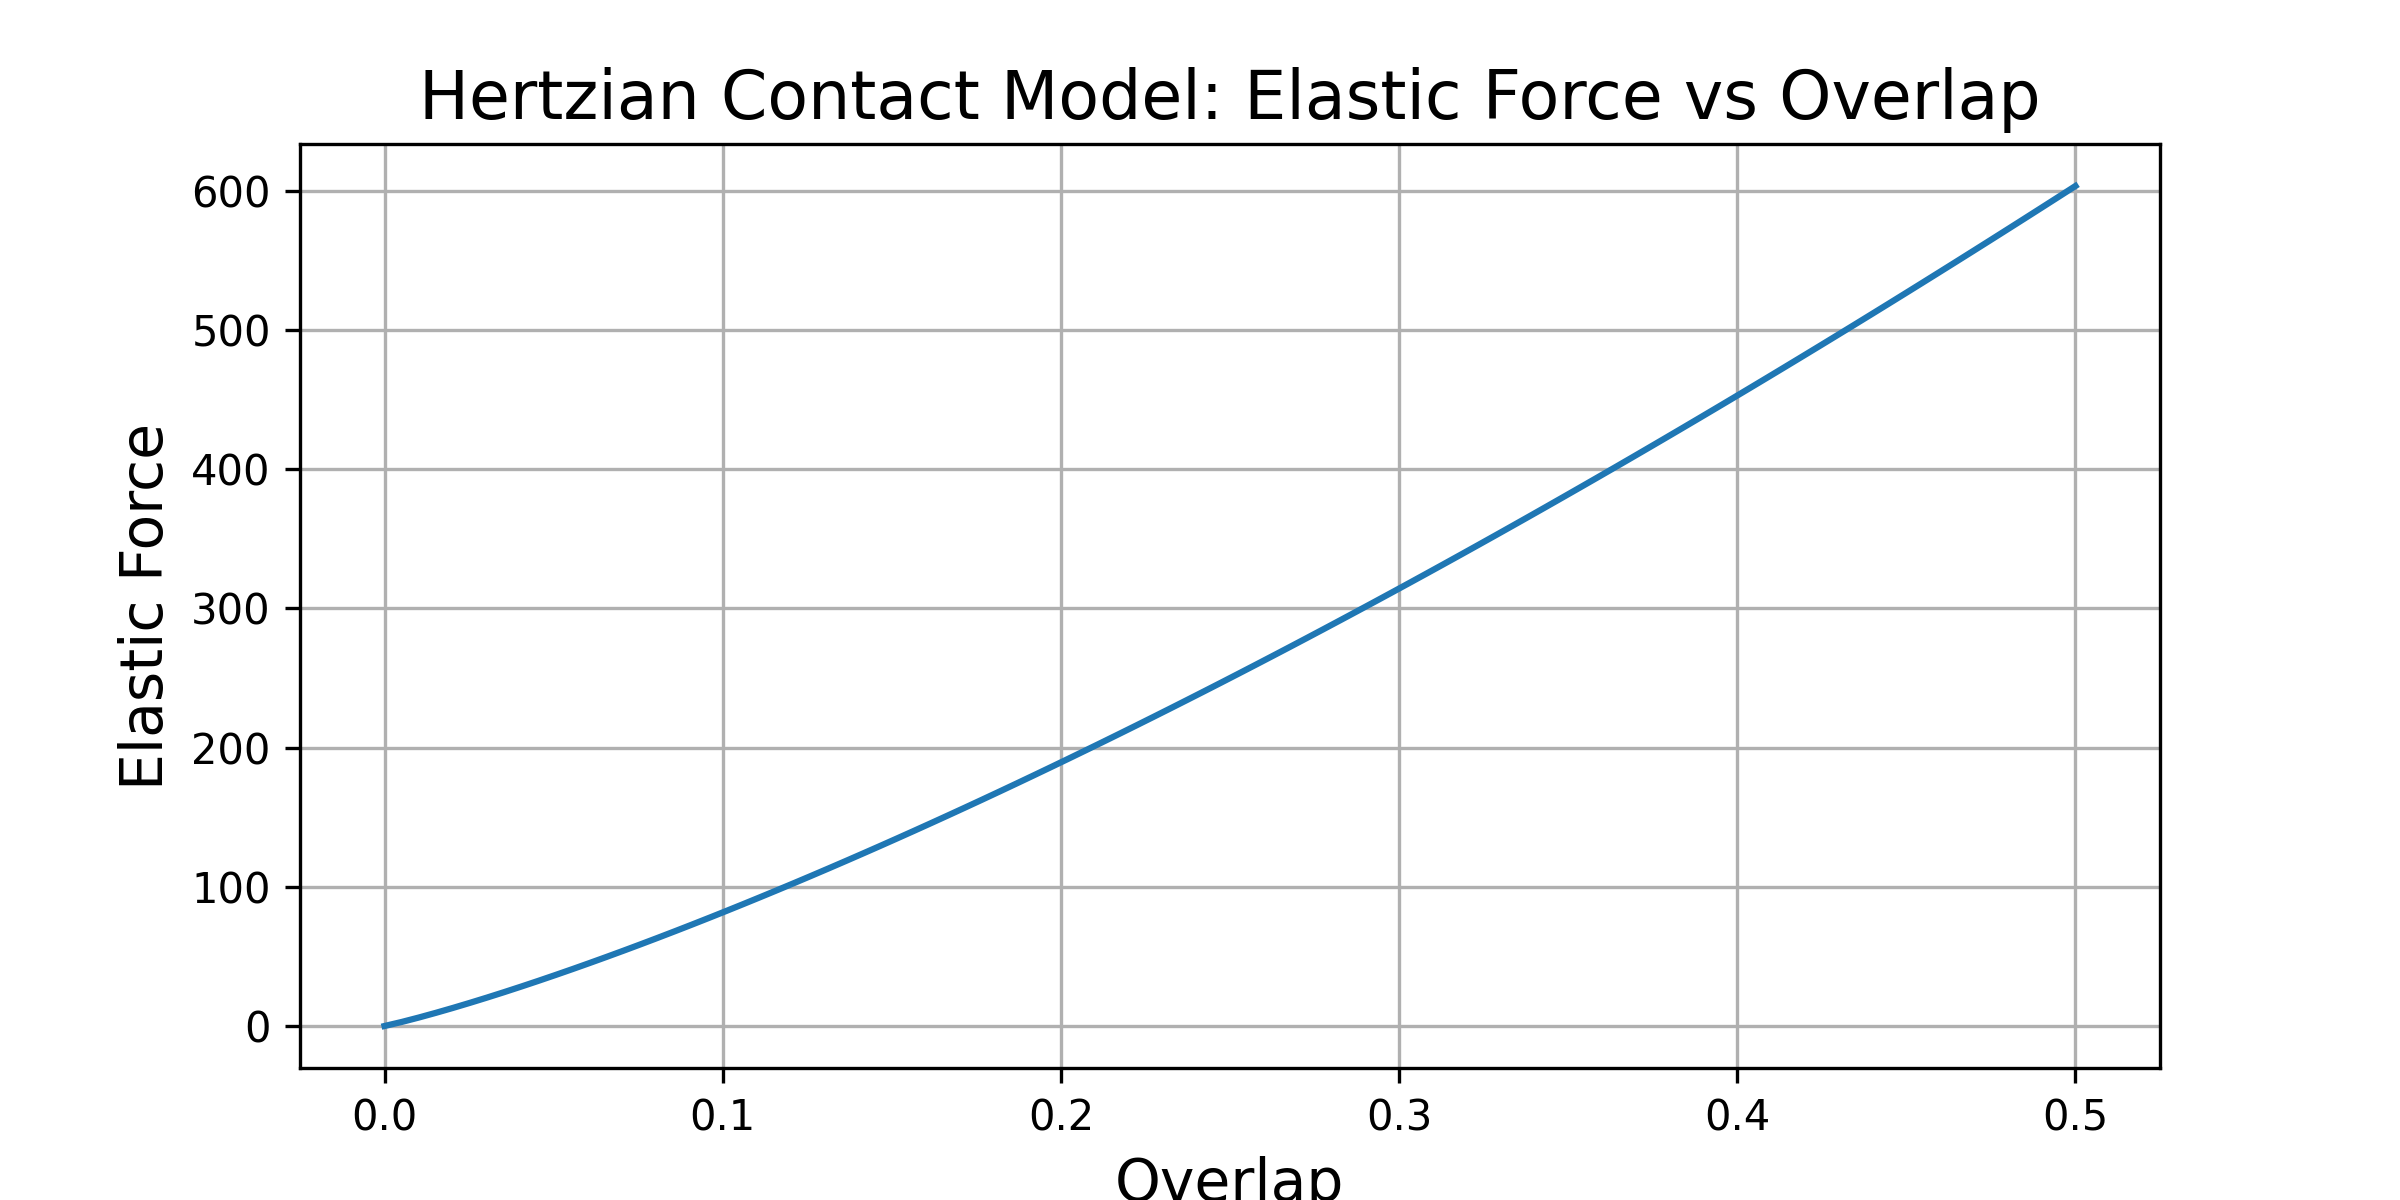
\includegraphics[width=\linewidth]{figures/hertzian_contact_model.png} % Slightly smaller width often looks better
    \caption{Force response of the Hertzian contact model. The repulsive force $\mathbf{F}^{\text{elastic}}$ scales non-linearly with the overlap distance, leading to a smooth increase in repulsion.}
    \label{fig:hertzian_contact_model}
\end{figure}

\subsection{Hard Collision Model}


The hard collision model enforces strict non-overlapping constraints between cells using a constraint-based method. For each pair of nearby cells, we define a constraint $\alpha$ based on the two closest points, $\mathbf{y}_n$ and $\mathbf{y}_m$, on their respective surfaces.

Contrary to the soft model (\autoref{eq:hertzian_contact_model}), where force is a direct function of overlap, the hard model defines the force and torque contributions from each constraint in terms of an unknown scalar magnitude $\gamma_\alpha$. This Lagrange multiplier represents the magnitude of the impulse required to prevent penetration. The force exerted on cell $n$ due to constraint $\alpha$ is:

\begin{equation} \label{eq:constraint_force}
    \mathbf{F}^{hard}_{n\alpha} = \hat{\mathbf{n}}_\alpha \gamma_\alpha
\end{equation}


where $\hat{\mathbf{n}}_\alpha$ is the normal vector at the contact point. The corresponding torque is $\boldsymbol{\tau}_{n\alpha} = (\mathbf{y}_n - \mathbf{x}_n) \times \hat{\mathbf{n}}_\alpha \gamma_\alpha$.

We collect all $C$ constraint multipliers into a single vector $\boldsymbol{\gamma} = [\dots, \gamma_\alpha, \dots]^T \in \mathbb{R}^{C}$. The total generalized force vector $\mathbfcal{F}$ for the colony, encompassing forces and torques on all cells, depends linearly on these multipliers and can be expressed as:
\begin{equation}
    \mathbfcal{F}(\boldsymbol{\gamma}) = \mathbfcal{D} \boldsymbol{\gamma}
\end{equation}
Here, $\mathbfcal{D} \in \mathbb{R}^{6N \times C}$ is a sparse matrix that maps the constraint multipliers to the resultant forces and torques on each cell. Each column of $\mathbfcal{D}$ corresponds to a constraint $\alpha$ and contains the normal vector $\hat{\mathbf{n}}_\alpha$ and the cross product $(\mathbf{y}_n - \mathbf{x}n) \times \hat{\mathbf{n}}\alpha$ for the involved cells, implementing the effect described by \autoref{eq:constraint_force}.

\subsubsection{Constraint Resolution}

The goal is to solve for the multipliers $\boldsymbol{\gamma}$ such that all overlaps are resolved. We require that these forces are strictly repulsive, which implies the multipliers must be non-negative:
\begin{align}
    \boldsymbol{\gamma} \geq 0
\end{align}

Let $\mathbf{\Phi}^k = [\dots, \Phi_\alpha, \dots]^T \in \mathbb{R}^{C}$ be the vector of signed separation distances for each constraint at time step $k$, where $\Phi_\alpha < 0$ indicates penetration. The non-overlap condition requires that after applying the forces, all constraints are satisfied:
\begin{align}
    \mathbf{\Phi}^{k+1} \geq 0
\end{align}

Furthermore, a complementarity condition must hold: a constraint can only generate a repulsive force ($\gamma_\alpha > 0$) if the cells are exactly in contact ($\Phi_\alpha^{k+1} = 0$) after the update. Conversely, if cells are separated ($\Phi_\alpha^{k+1} > 0$), the corresponding force must be zero. This is expressed as:
\begin{align}
    \boldsymbol{\gamma}^T \mathbf{\Phi}^{k+1} = 0 \quad \text{or, equivalently,} \quad \boldsymbol{\gamma} \perp \mathbf{\Phi}^{k+1}
\end{align}
These three conditions are often abbreviated as

\begin{equation}
    \mathbf{0} \leq \boldsymbol{\gamma} \perp \mathbf{\Phi}^{k+1} \geq \mathbf{0}
\end{equation}


The colony update rule from \autoref{eq:colony_update} and the constraint conditions can now be combined:

\begin{align}
    \mathbfcal{C}^{k+1}          & = \mathbfcal{C}^k + \Delta t \, \mathbfcal{G} \mathbfcal{M} \mathbfcal{D} \boldsymbol{\gamma} \label{eq:hard_update_constraint} \\
    \text{s.t.} \quad \mathbf{0} & \leq \boldsymbol{\gamma} \perp \mathbf{\Phi}^{k+1} \geq \mathbf{0} \label{eq:hard_constraints}
\end{align}

The central challenge is that $\mathbf{\Phi}^{k+1}$ is a nonlinear function of the updated state $\mathbfcal{C}^{k+1}$, which itself depends on $\boldsymbol{\gamma}$. Weady et al.\cite{Weady2024} linearize this relationship using a first-order Taylor expansion around the current state $\mathbfcal{C}^k$:

\begin{align}
    \mathbf{\Phi}^{k+1} & \approx \mathbf{\Phi}^k + \Delta t \left( \mathbfcal{D}^T \dot{\mathbfcal{C}}^k - \mathbfcal{L}^T\dot{\boldsymbol{\ell}^k} \right)                                                            \\
                        & = \mathbf{\Phi}^k + \Delta t \left( \mathbfcal{D}^T \mathbfcal{G} \mathbfcal{M} \mathbfcal{D} \boldsymbol{\gamma} - \mathbfcal{L}^T \dot{\boldsymbol{\ell}^k} \right) \label{eq:phi_expanded}
\end{align}

The change in separation distances depends on two factors:

\begin{enumerate}
    \item \textbf{Cell Motion:} The term $\mathbfcal{D}^T \mathbfcal{G} \mathbfcal{M} \mathbfcal{D} \boldsymbol{\gamma}$ represents how constraint forces induce motion that changes $\mathbf{\Phi}$.
    \item \textbf{Cell Growth:} The term $\mathbfcal{L}^T \dot{\boldsymbol{\ell}}^k$ accounts for how independent cell growth $\dot{\boldsymbol{\ell}}^k$ affects the separation distances. The matrix $\mathbfcal{L} \in \mathbb{R}^{N \times C}$ encodes the sensitivity of each constraint $\alpha$ to the growth of each cell $n$.  Note that $\dot{\boldsymbol{\ell}}^k$ is calculated using \autoref{eq:growth} and depends itself on $\boldsymbol{\gamma}$.
\end{enumerate}

Substituting the linearized approximation \autoref{eq:phi_expanded} into the complementarity condition \autoref{eq:hard_constraints} yields a standard Linear Complementarity Problem (LCP):

\begin{equation}  \label{eq:final_lcp}
    \begin{aligned}
         & \text{Find } \boldsymbol{\gamma} \text{ such that} \\
         & \mathbf{0} \leq \boldsymbol{\gamma}
        \;\perp\;
        \mathbf{\Phi}^k
        + \Delta t \left( \mathbfcal{D}^T \mathbfcal{G} \mathbfcal{M} \mathbfcal{D}\,\boldsymbol{\gamma}
        - \mathbfcal{L}^T \dot{\boldsymbol{\ell}}^k \right)
        \geq \mathbf{0}
    \end{aligned}
\end{equation}

This LCP can be solved efficiently for $\boldsymbol{\gamma}$ using specialized algorithms like the Barzilai-Borwein Projected Gradient Descent (BBPGD) method as described in \cite{Weady2024}. The solution $\boldsymbol{\gamma}$ is then used to compute the constraint forces $\mathbfcal{F}(\boldsymbol{\gamma})$ and update the colony state via \autoref{eq:hard_update_constraint}.


Weady et al. \cite{Weady2024} further enhance this basic scheme with a recursive iterative solver to correct for violations caused by the first-order linearization, ensuring strict non-overlap. We refer the reader to their supplementary material for a comprehensive description of the full, robust algorithm which we have implemented in our framework.

\newpage

\section{Implementation}

All simulations in this paper were performed with a custom C++ framework developed for large-scale simulations of proliferating cell collectives. The framework is designed for distributed-memory parallel computing and leverages standard HPC libraries to ensure scalability and efficiency. Its core components are:

\subsection{Distributed Computing Architecture}

The core architecture is built on two foundational libraries:
\begin{itemize}
    \item PETSc\cite{petsc-web-page}, used as a backend for distributed vectors and sparse matrices. PETSc partitions data across MPI processes, transparently handling inter-process communication so that global operations (e.g., matrix-vector products, reductions) can be expressed at a high level.
    \item MPI, which underlies all inter-process communication, including ghost-cell exchanges at domain boundaries to enable consistent collision handling across partitions.
\end{itemize}

On top of these abstractions, the framework implements the full physics pipeline, including the BBPGD solver for the hard collision model \cite{Weady2024} and the soft collision model.


\subsection{Collision Handling Pipeline}

Collisions are processed through a unified pipeline. A spatial grid enables broad-phase detection, reducing neighbor searches to $O(N)$, followed by narrow-phase detection that computes exact contact points. For each collision, the framework assembles a standardized data package containing:

\begin{itemize}
    \item Contact point in world coordinates.
    \item Normal vector $\hat{\mathbf{n}}$ at the contact.
    \item Torque arms from the contact point to each cell center.
    \item Overlap distance $\delta$ (soft model).
    \item Unique identifiers of the two cells.
\end{itemize}

This abstraction decouples geometry from physics: both collision models consume the same data structure but compute the resulting forces differently. This design allows easy extension to new collision models in the future.

\subsection{Simulation Output}

Simulation results are written in \texttt{VTK} format, which can be directly visualized with ParaView\cite{ahrens2005paraview}. This includes both raw particle and field data, as well as derived quantities such as contact forces or stresses.
All figures presented in the following sections, together with the data used for plots, were extracted from these ParaView outputs. This workflow ensures consistency between visualizations and quantitative analysis, while also enabling interactive inspection of the simulated cell collectives.


\subsection{Availability}

The full simulation framework, including all features and implementations described in this work, is openly available on GitHub at \url{https://github.com/manuellerchner/MicrobeGrowthSim-IDP}.
The repository enables reproduction of the presented results as well as adaptation of the framework for related research problems.

\subsection{Pattern Formation Analysis}

\subsubsection{Concentric Ring Patterns}

We begin by validating our implementations through the reproduction of concentric ring patterns that arise under stress-sensitive growth, as reported in \cite{Weady2024}. Simulations were performed for $\lambda = 10^{-1}, 10^{-2}, 10^{-3}$ using both hard and soft collision models. As shown in \autoref{fig:pattern_formation}, both models successfully produce qualitatively similar ring structures. This demonstrates that the soft collision model, despite its simpler formulation, can capture the essential dynamics responsible for these macroscopic patterns, making it a viable and potentially more efficient option for studying pattern formation.

Importantly, the soft model reproduces the expected concentric rings while employing a substantially simplified approach to collision resolution. This further supports its suitability as an alternative to the more complex hard collision model when the goal is to replicate such emergent patterns.



\subsubsection{Microdommain formation}

\cite{You2018}


\subsection{Quantitative Comparison}

To provide a more quantitative assessment, we analyze three key metrics: the radial distribution of stress, the radial distribution of packing fraction, and the maximum particle overlap over time. These metrics offer insights into the mechanical state of the colony and how it evolves under different collision models.

\autoref{fig:dense_packing_comparison} and \autoref{fig:radial_distribution_stress}--\autoref{fig:max_overlap_simulation} illustrate these results in detail While certain quantities, such as the packing fraction and the corresponding maximum overlap, differ between the two models, the overall macroscopic behavior remains similar, consistent with the pattern formation observed in \autoref{fig:pattern_formation}.

\begin{figure}[H]
    \centering
    \begin{subfigure}[b]{0.49\columnwidth}
        \centering
        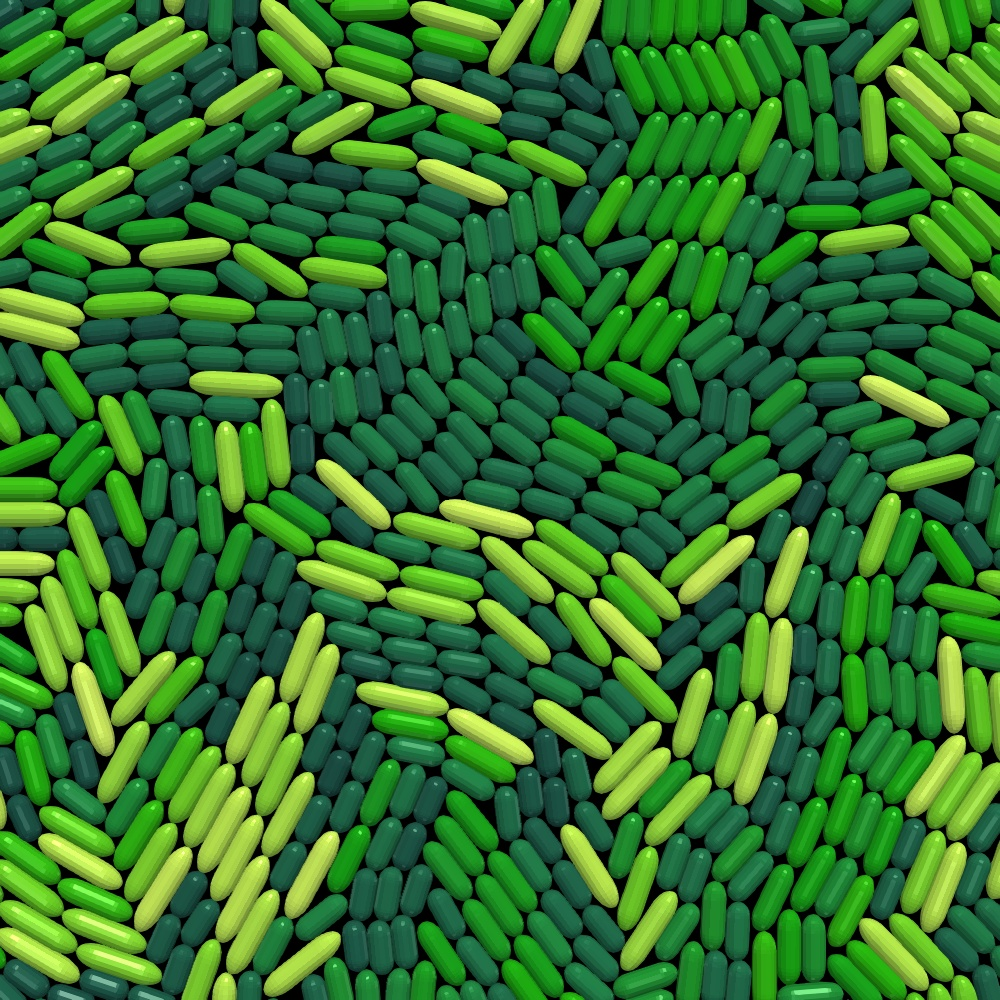
\includegraphics[width=\linewidth]{figures/comparisons/packing_hard.jpeg}
        \caption{Close-up of particle packing for the hard model.}
        \label{fig:packing_hard}
    \end{subfigure}
    \begin{subfigure}[b]{0.49\columnwidth}
        \centering
        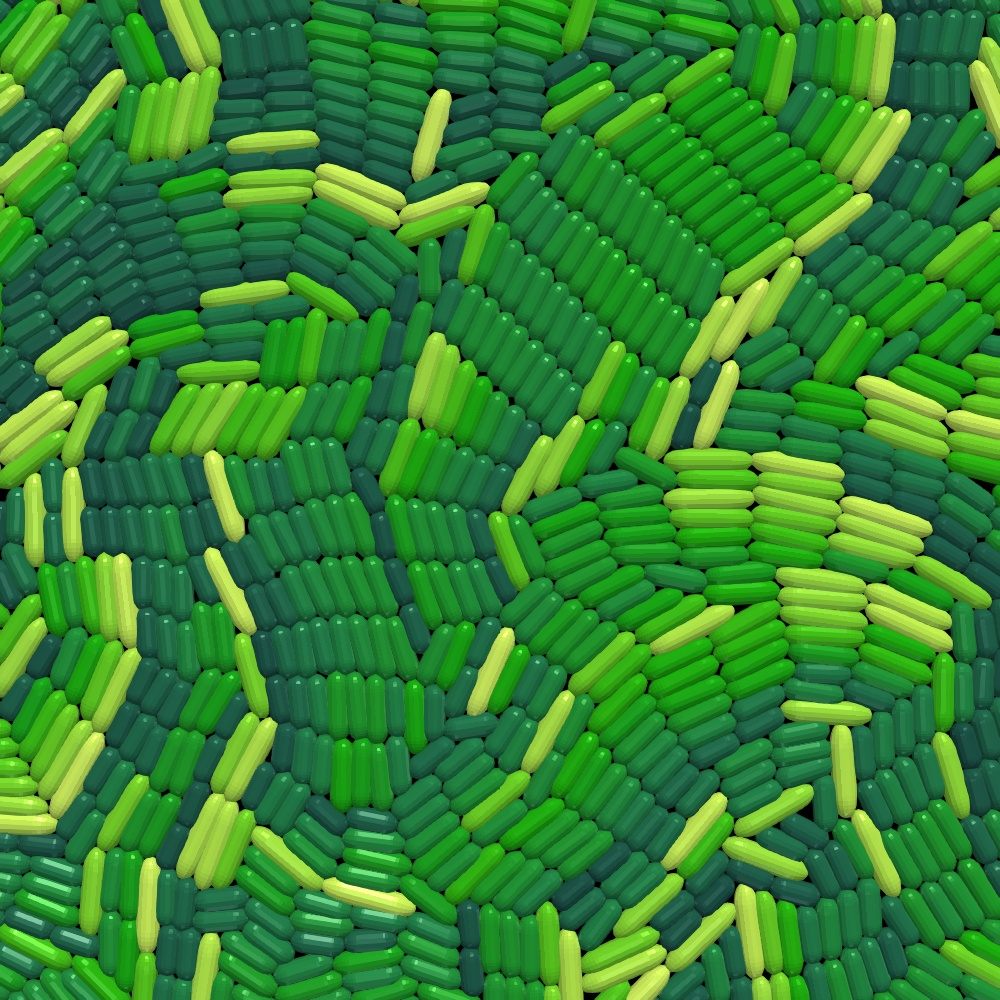
\includegraphics[width=\linewidth]{figures/comparisons/packing_soft.jpeg}
        \caption{Close-up of particle packing for the soft model.}
        \label{fig:packing_soft}
    \end{subfigure}
    \caption{Close-up comparison of particle packing. The soft model exhibits denser packing with slight particle overlap, while the hard model maintains strict non-overlap. See \autoref{fig:radial_distribution_packing_fraction} for a quantitative comparison of packing fractions.}
    \label{fig:dense_packing_comparison}
\end{figure}



\newpage

\begin{figure}[H]
    \centering
    \begin{subfigure}[b]{\linewidth}
        \centering
        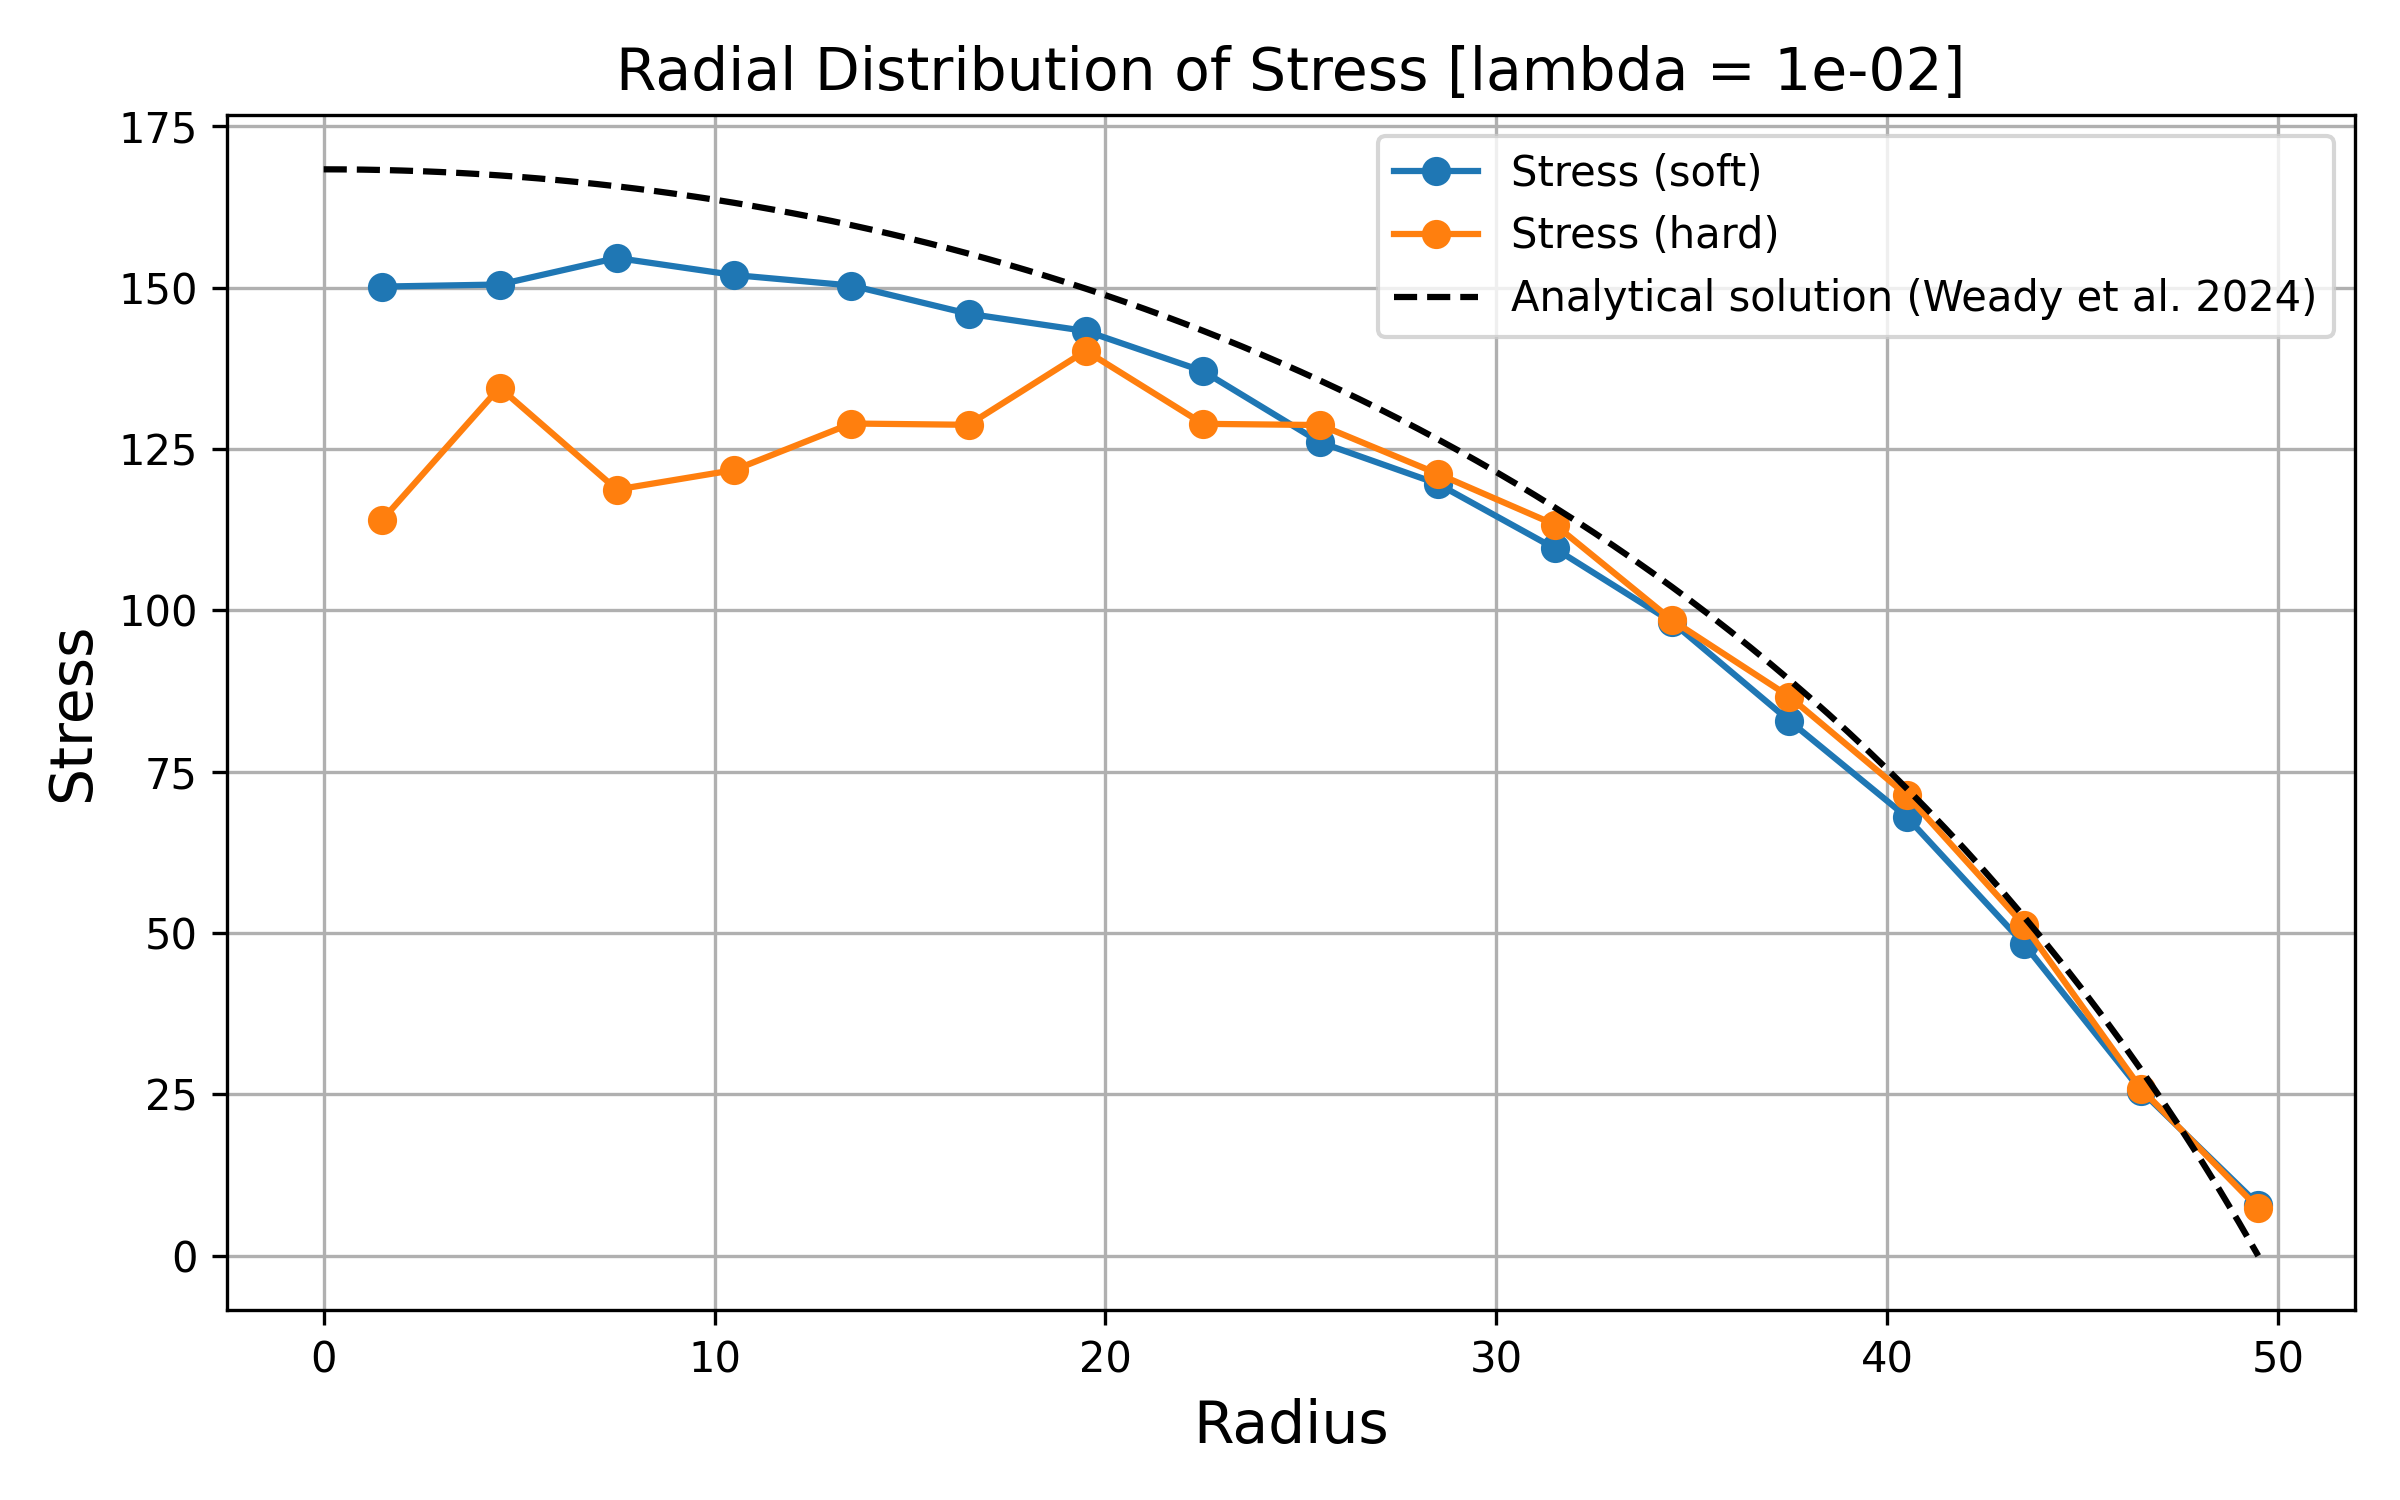
\includegraphics[width=\linewidth]{figures/comparisons/radial_distribution_stress.png}
        \caption{Comparison of radial stress distributions for the hard and soft collision models. Both models roughly reproduce the analytically derived stress profiles \cite{Weady2024}.}
        \label{fig:radial_distribution_stress}
    \end{subfigure}

    \vspace{0.5em}

    \begin{subfigure}[b]{\linewidth}
        \centering
        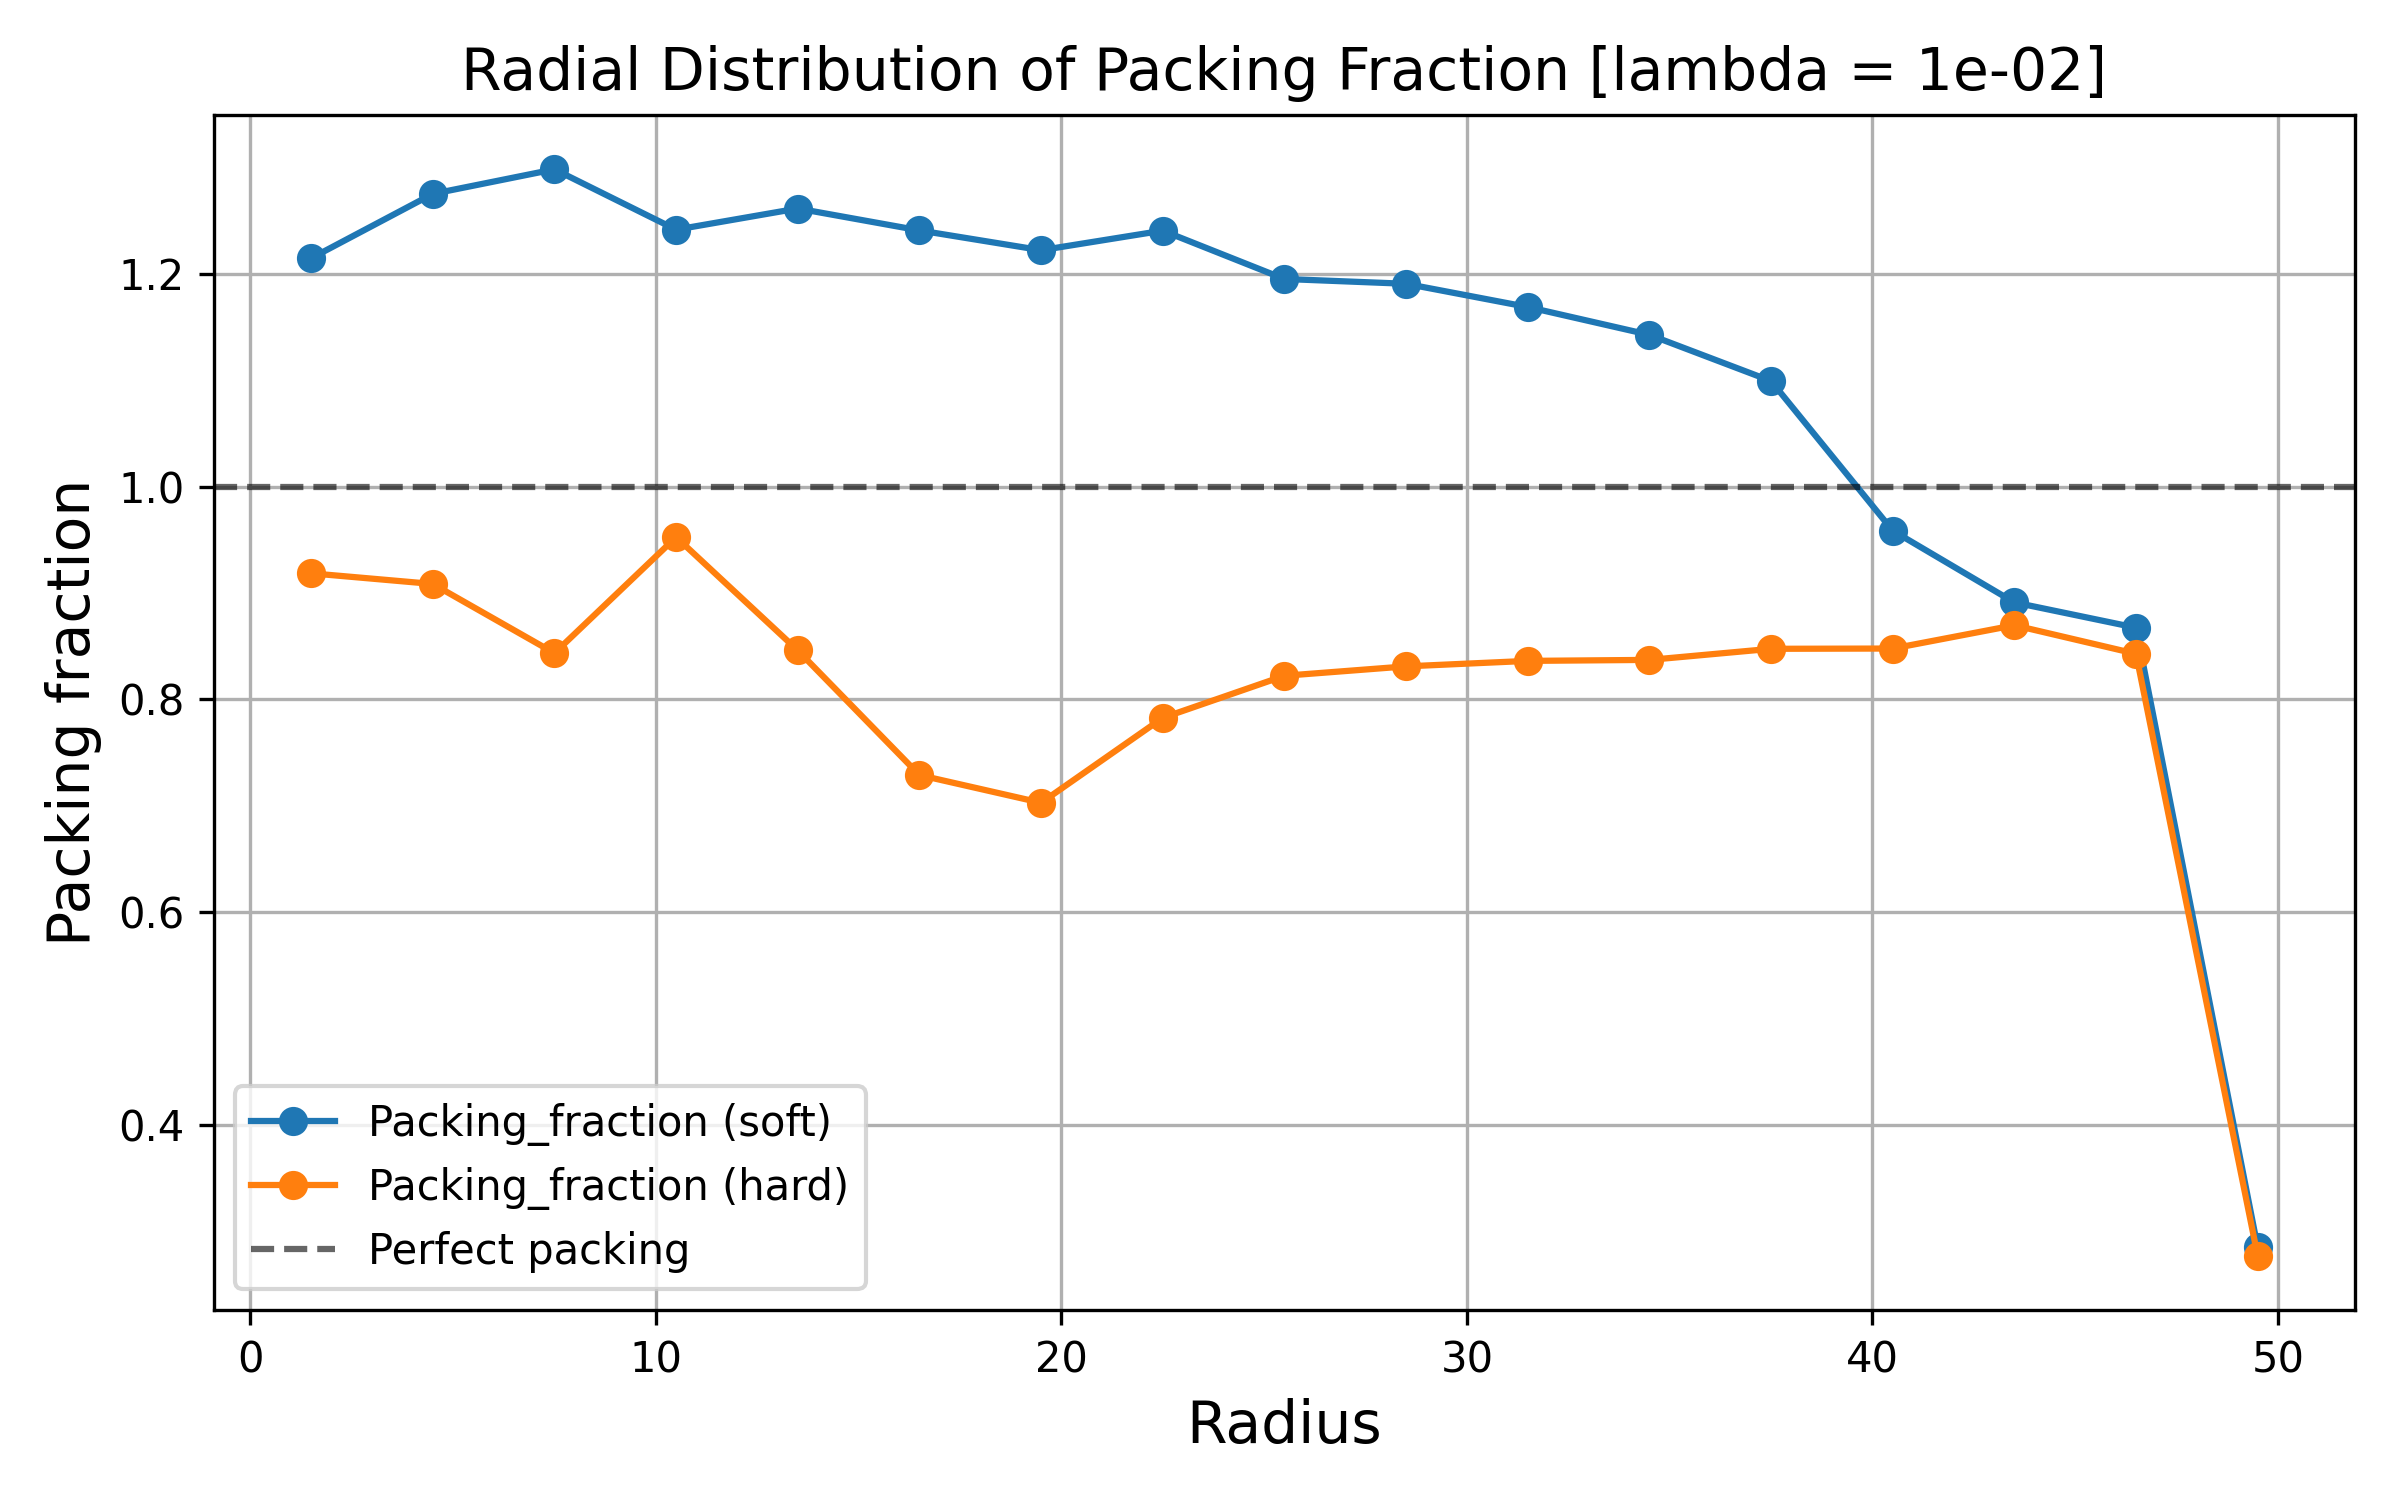
\includegraphics[width=\linewidth]{figures/comparisons/radial_distribution_packing_fraction.png}
        \caption{Radial packing fraction. The soft model reaches $\approx1.2$ at the center due to overlap, while the hard model stays below 1. The packing fraction is defined as the total area occupied by particles within a radial shell divided by the shell area.}
        \label{fig:radial_distribution_packing_fraction}
    \end{subfigure}

    \vspace{0.5em}

    \begin{subfigure}[b]{\linewidth}
        \centering
        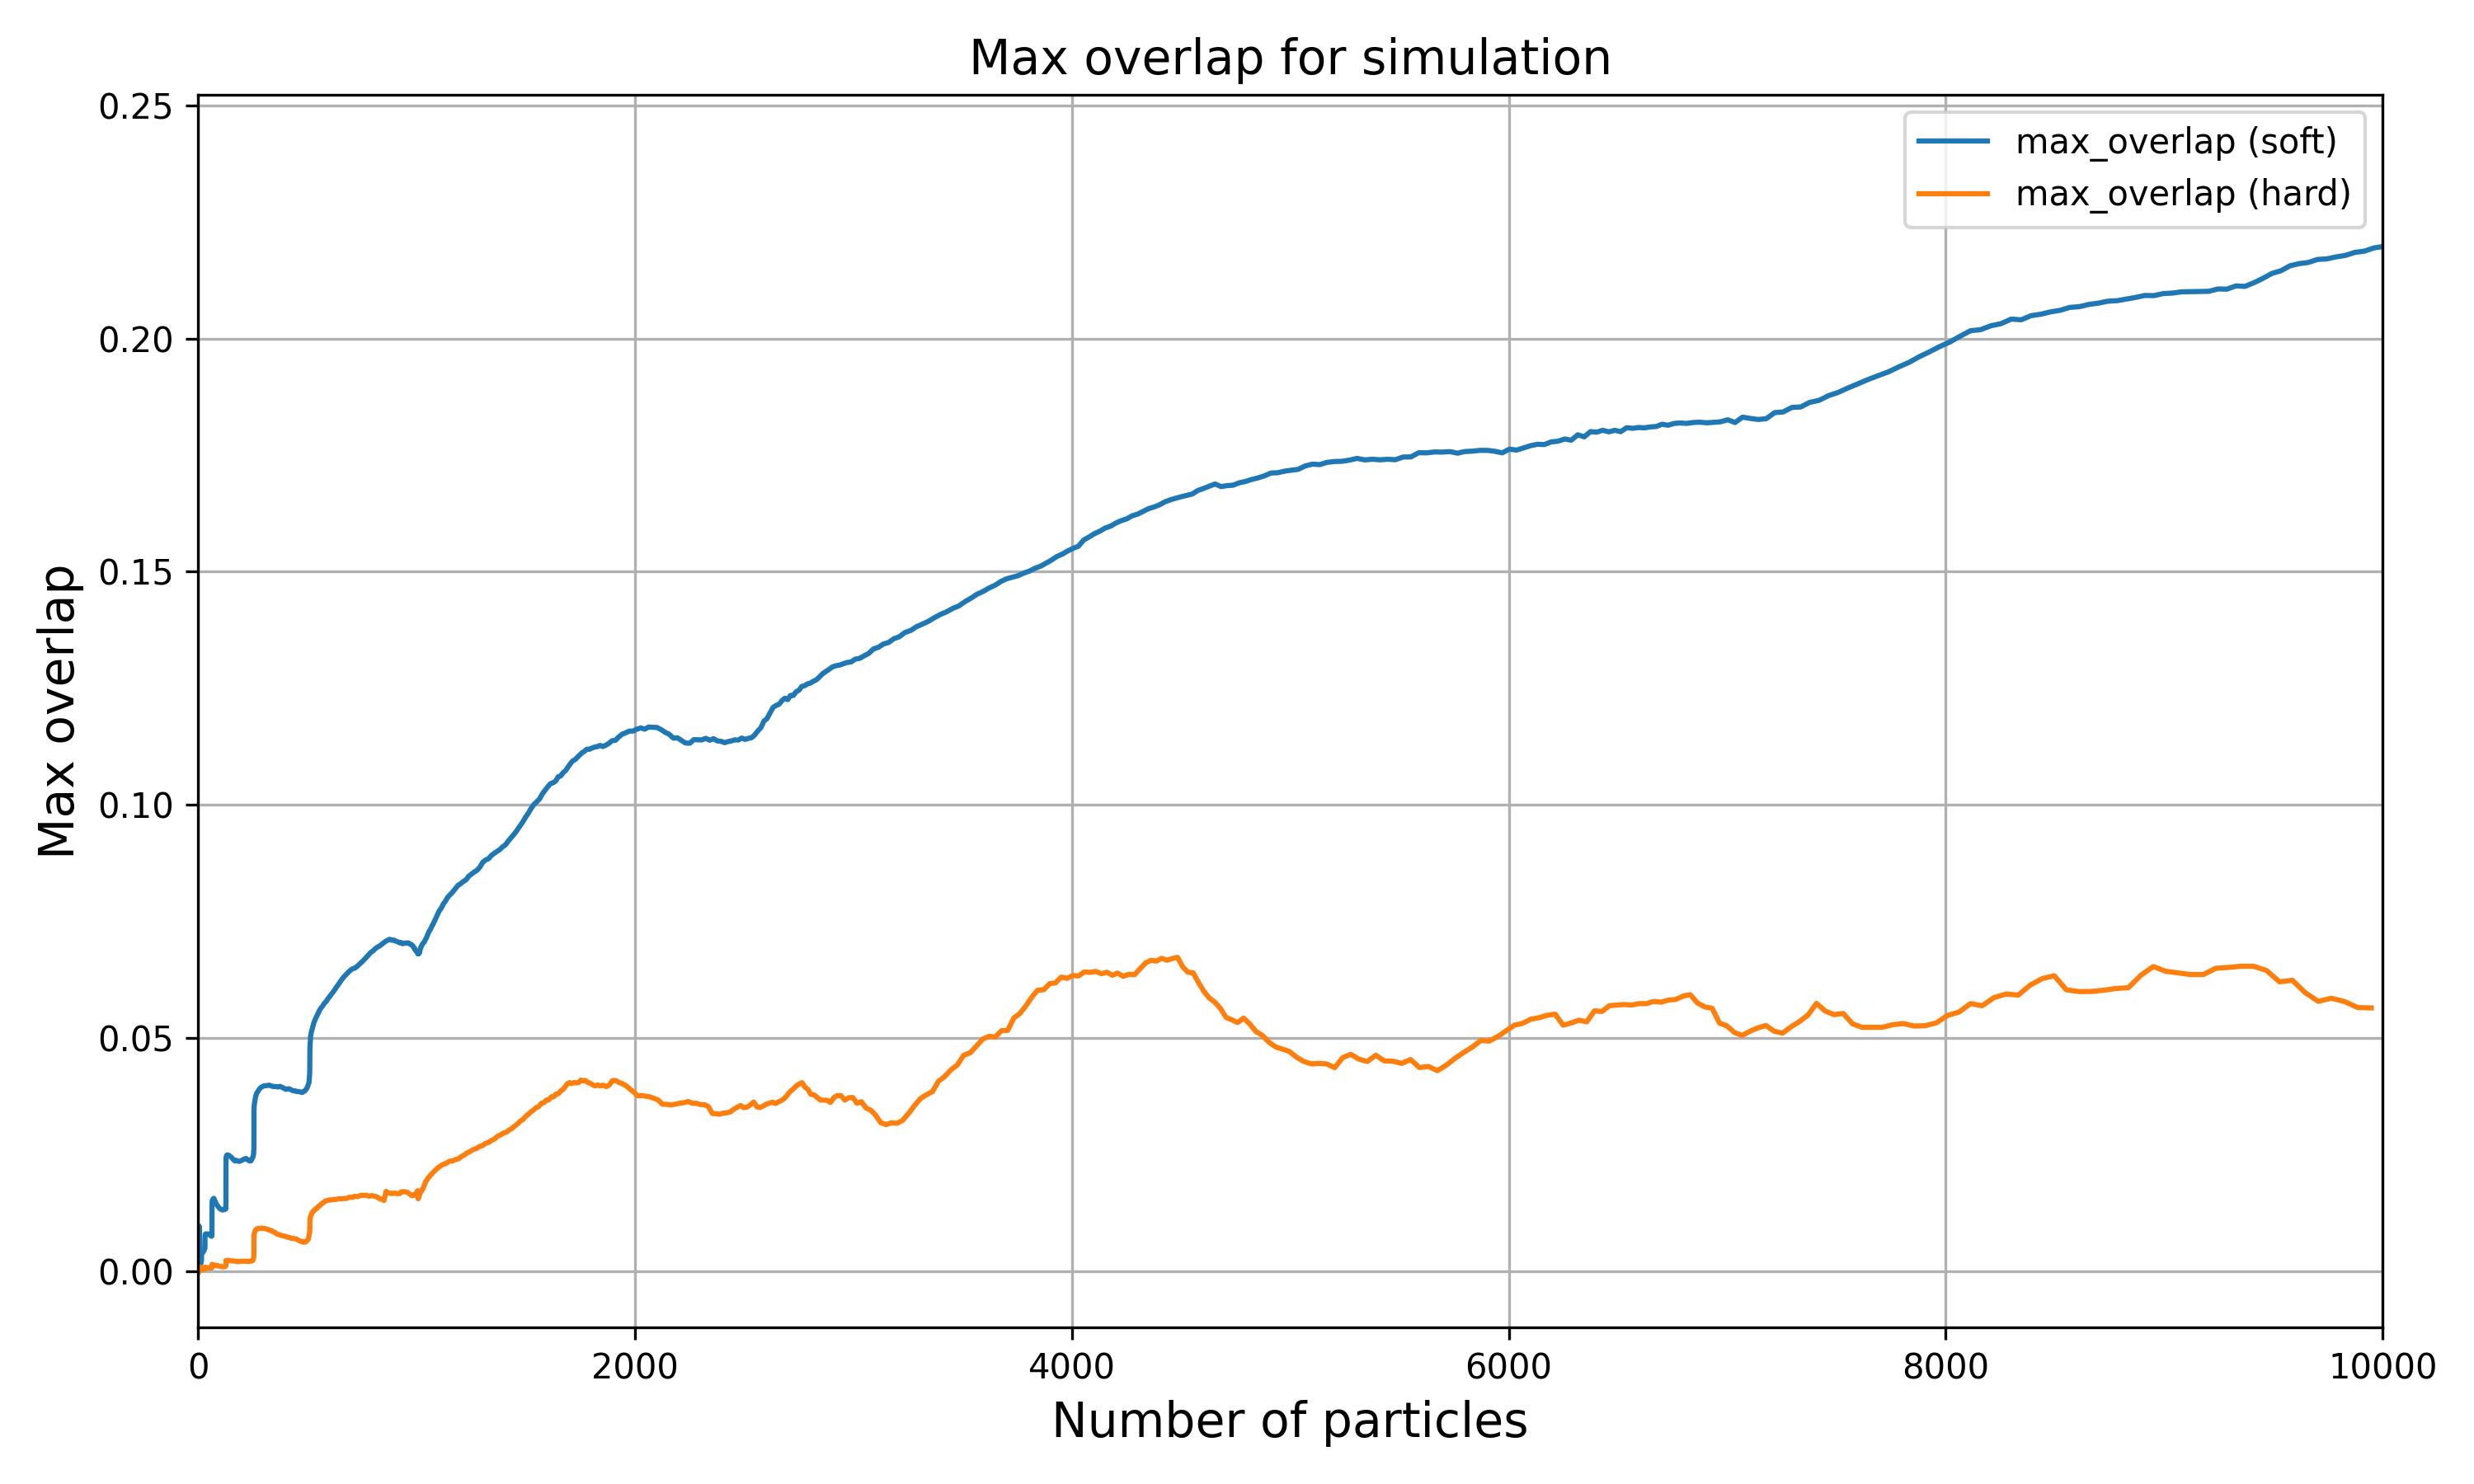
\includegraphics[width=\linewidth]{figures/comparisons/max_overlap_simulation.png}
        \caption{Maximum particle overlap. Overlap grows over time in the soft model, while the hard model is kept near a constant value set by the tolerance hyperparameter.}
        \label{fig:max_overlap_simulation}
    \end{subfigure}

    \caption{Comparison of hard and soft collision models: (a) radial stress distributions, (b) radial packing fraction, and (c) maximum particle overlap.}
    \label{fig:comparison_all}
\end{figure}

\begin{figure*}[p]
    \centering

    % Lambda = 10^-1 comparison
    \begin{subfigure}[b]{\textwidth}
        \centering
        \caption{Growth Comparison $\lambda=10^{-1}$}
        \begin{tabular}{r M{\subfigwidth} M{\subfigwidth} M{\subfigwidth} M{\subfigwidth}}
            \growthcomparisonrow{Hard}{1e-1}{0400}{0800}{1200}{1800}
            \growthcomparisonrow{Soft}{1e-1}{0400}{0800}{1200}{1800}
        \end{tabular}
    \end{subfigure}

    % % Lambda = 10^-2 comparison
    \begin{subfigure}[b]{\textwidth}
        \centering
        \caption{Growth Comparison $\lambda=10^{-2}$}
        \begin{tabular}{r M{\subfigwidth} M{\subfigwidth} M{\subfigwidth} M{\subfigwidth}}
            \growthcomparisonrow{Hard}{1e-2}{0400}{0700}{0900}{1100}
            \growthcomparisonrow{Soft}{1e-2}{0400}{0700}{0900}{1100}
        \end{tabular}
    \end{subfigure}

    % Lambda = 10^-3 comparison
    \begin{subfigure}[b]{\textwidth}
        \centering
        \caption{Growth Comparison $\lambda=10^{-3}$}
        \begin{tabular}{r M{\subfigwidth} M{\subfigwidth} M{\subfigwidth} M{\subfigwidth}}
            \growthcomparisonrow{Hard}{1e-3}{0400}{0600}{0800}{1000}
            \growthcomparisonrow{Soft}{1e-3}{0400}{0600}{0800}{1000}
        \end{tabular}
    \end{subfigure}


    \caption{Pattern formation under stress-sensitive growth at equally spaced time points. Each row shows the evolution for a different value of $\lambda$ for both hard and soft collision models up to a maximum colony radius of 50. The color indicates the length of the cells ranging from 1 (dark green) to 2 (light green). Clear concentric ring pattern are visible for $\lambda \in \{10^{-2}, 10^{-3}\}$.}
    \label{fig:pattern_formation}
\end{figure*}





\newpage

\section{Computational Performance}

While both models reproduce the observed patterns, our preliminary analysis suggests significant performance differences. The hard collision model's requirement to solve an LCP at each time step introduces a computational bottleneck, potentially limiting its scalability for very large systems or long simulation times. In contrast, the direct force calculation in the soft collision model is inherently less complex per interaction but typical needs to be computed using a finder time step to avoid instabilities.


Moreover solving a LCP requires global information about the system, as it is essentially optimizing a global system of constraints. This can lead to increased communication overhead in parallel implementations, as all processors take part in an iterative solver and are required to share information about all particles in the system during each optimization step.


In contrast, the soft collision model only requires local information about neighboring particles to compute forces, and can be efficiencyly computed using common molecular dynamics techniques such as cell lists or Verlet lists (See \cite{Gratl2019}). This locality greatly reduces the amount of inter-processor communication needed in a parallel implementation, as each processor can largely operate independently on its own subset of particles, only needing to occasionally exchange information about particles near the boundaries of its domain.


\begin{figure}
    \centering
    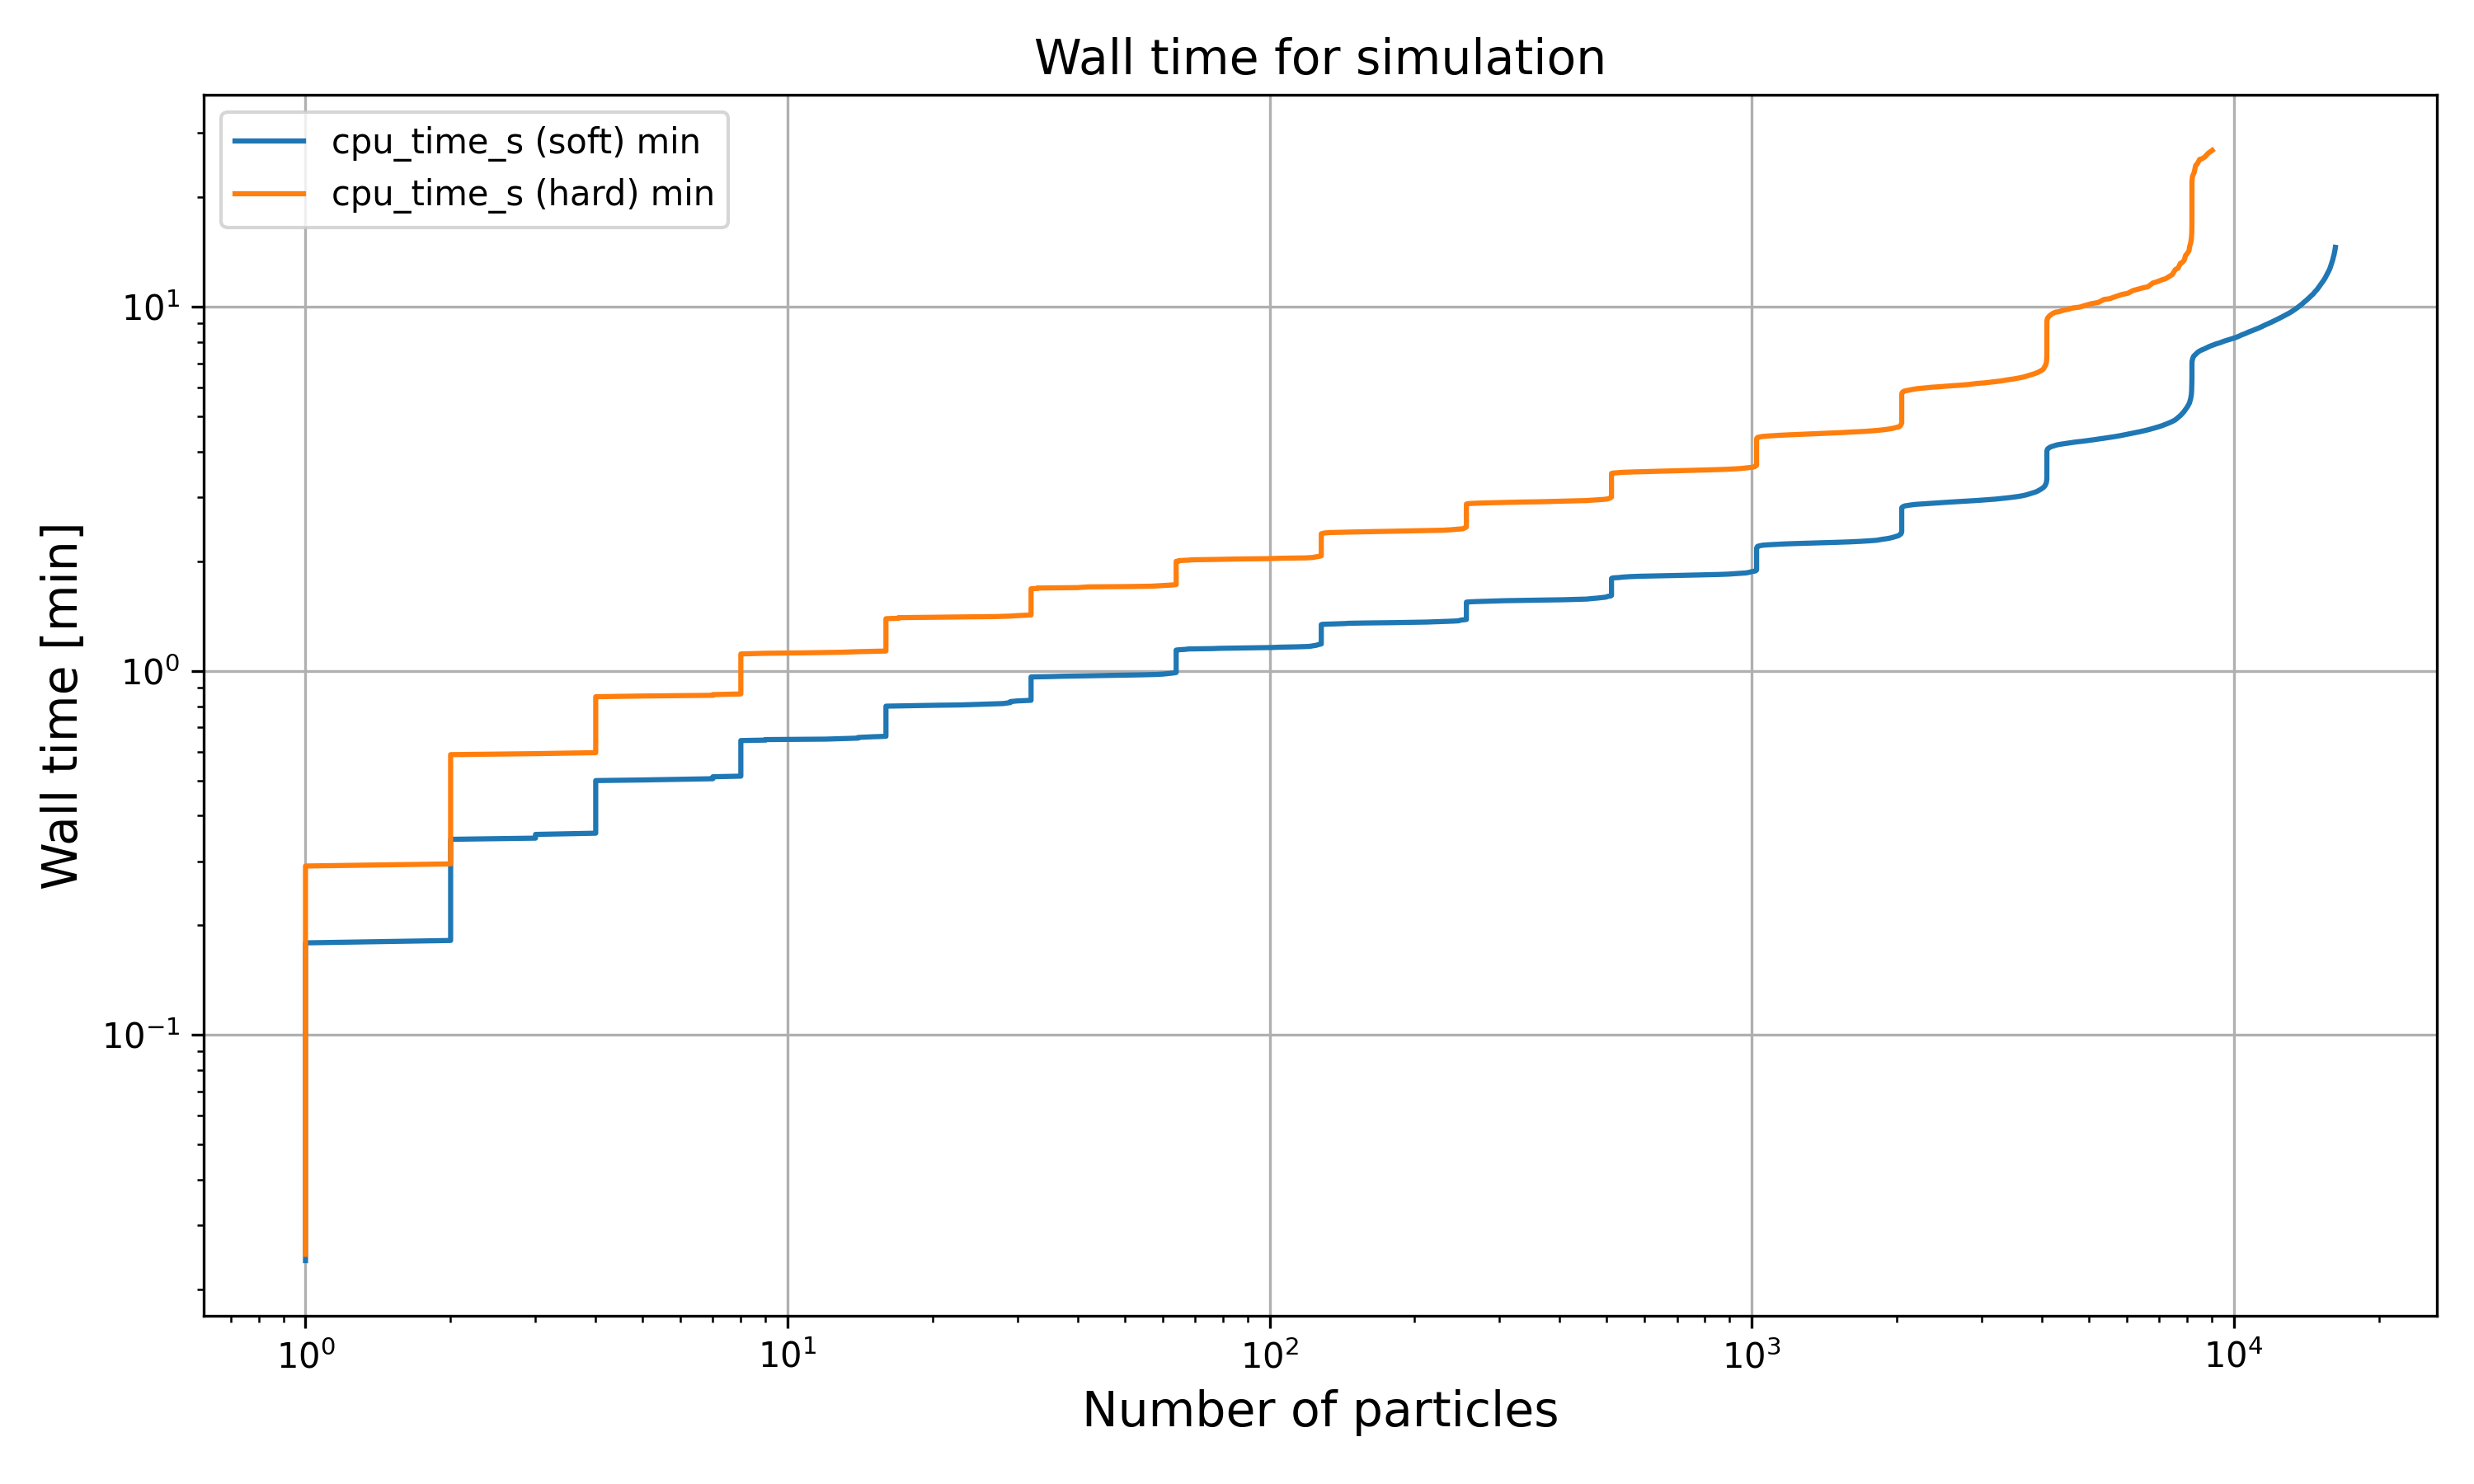
\includegraphics[width=\linewidth]{figures/comparisons/wall_time_simulation.png}
    \caption{Comparison of the total simulation time for the hard and soft collision models over number of particles. The soft model is generally faster by a factor of 1.8.}
    \label{figure:wall_time_simulation}
\end{figure}

\begin{figure}
    \centering
    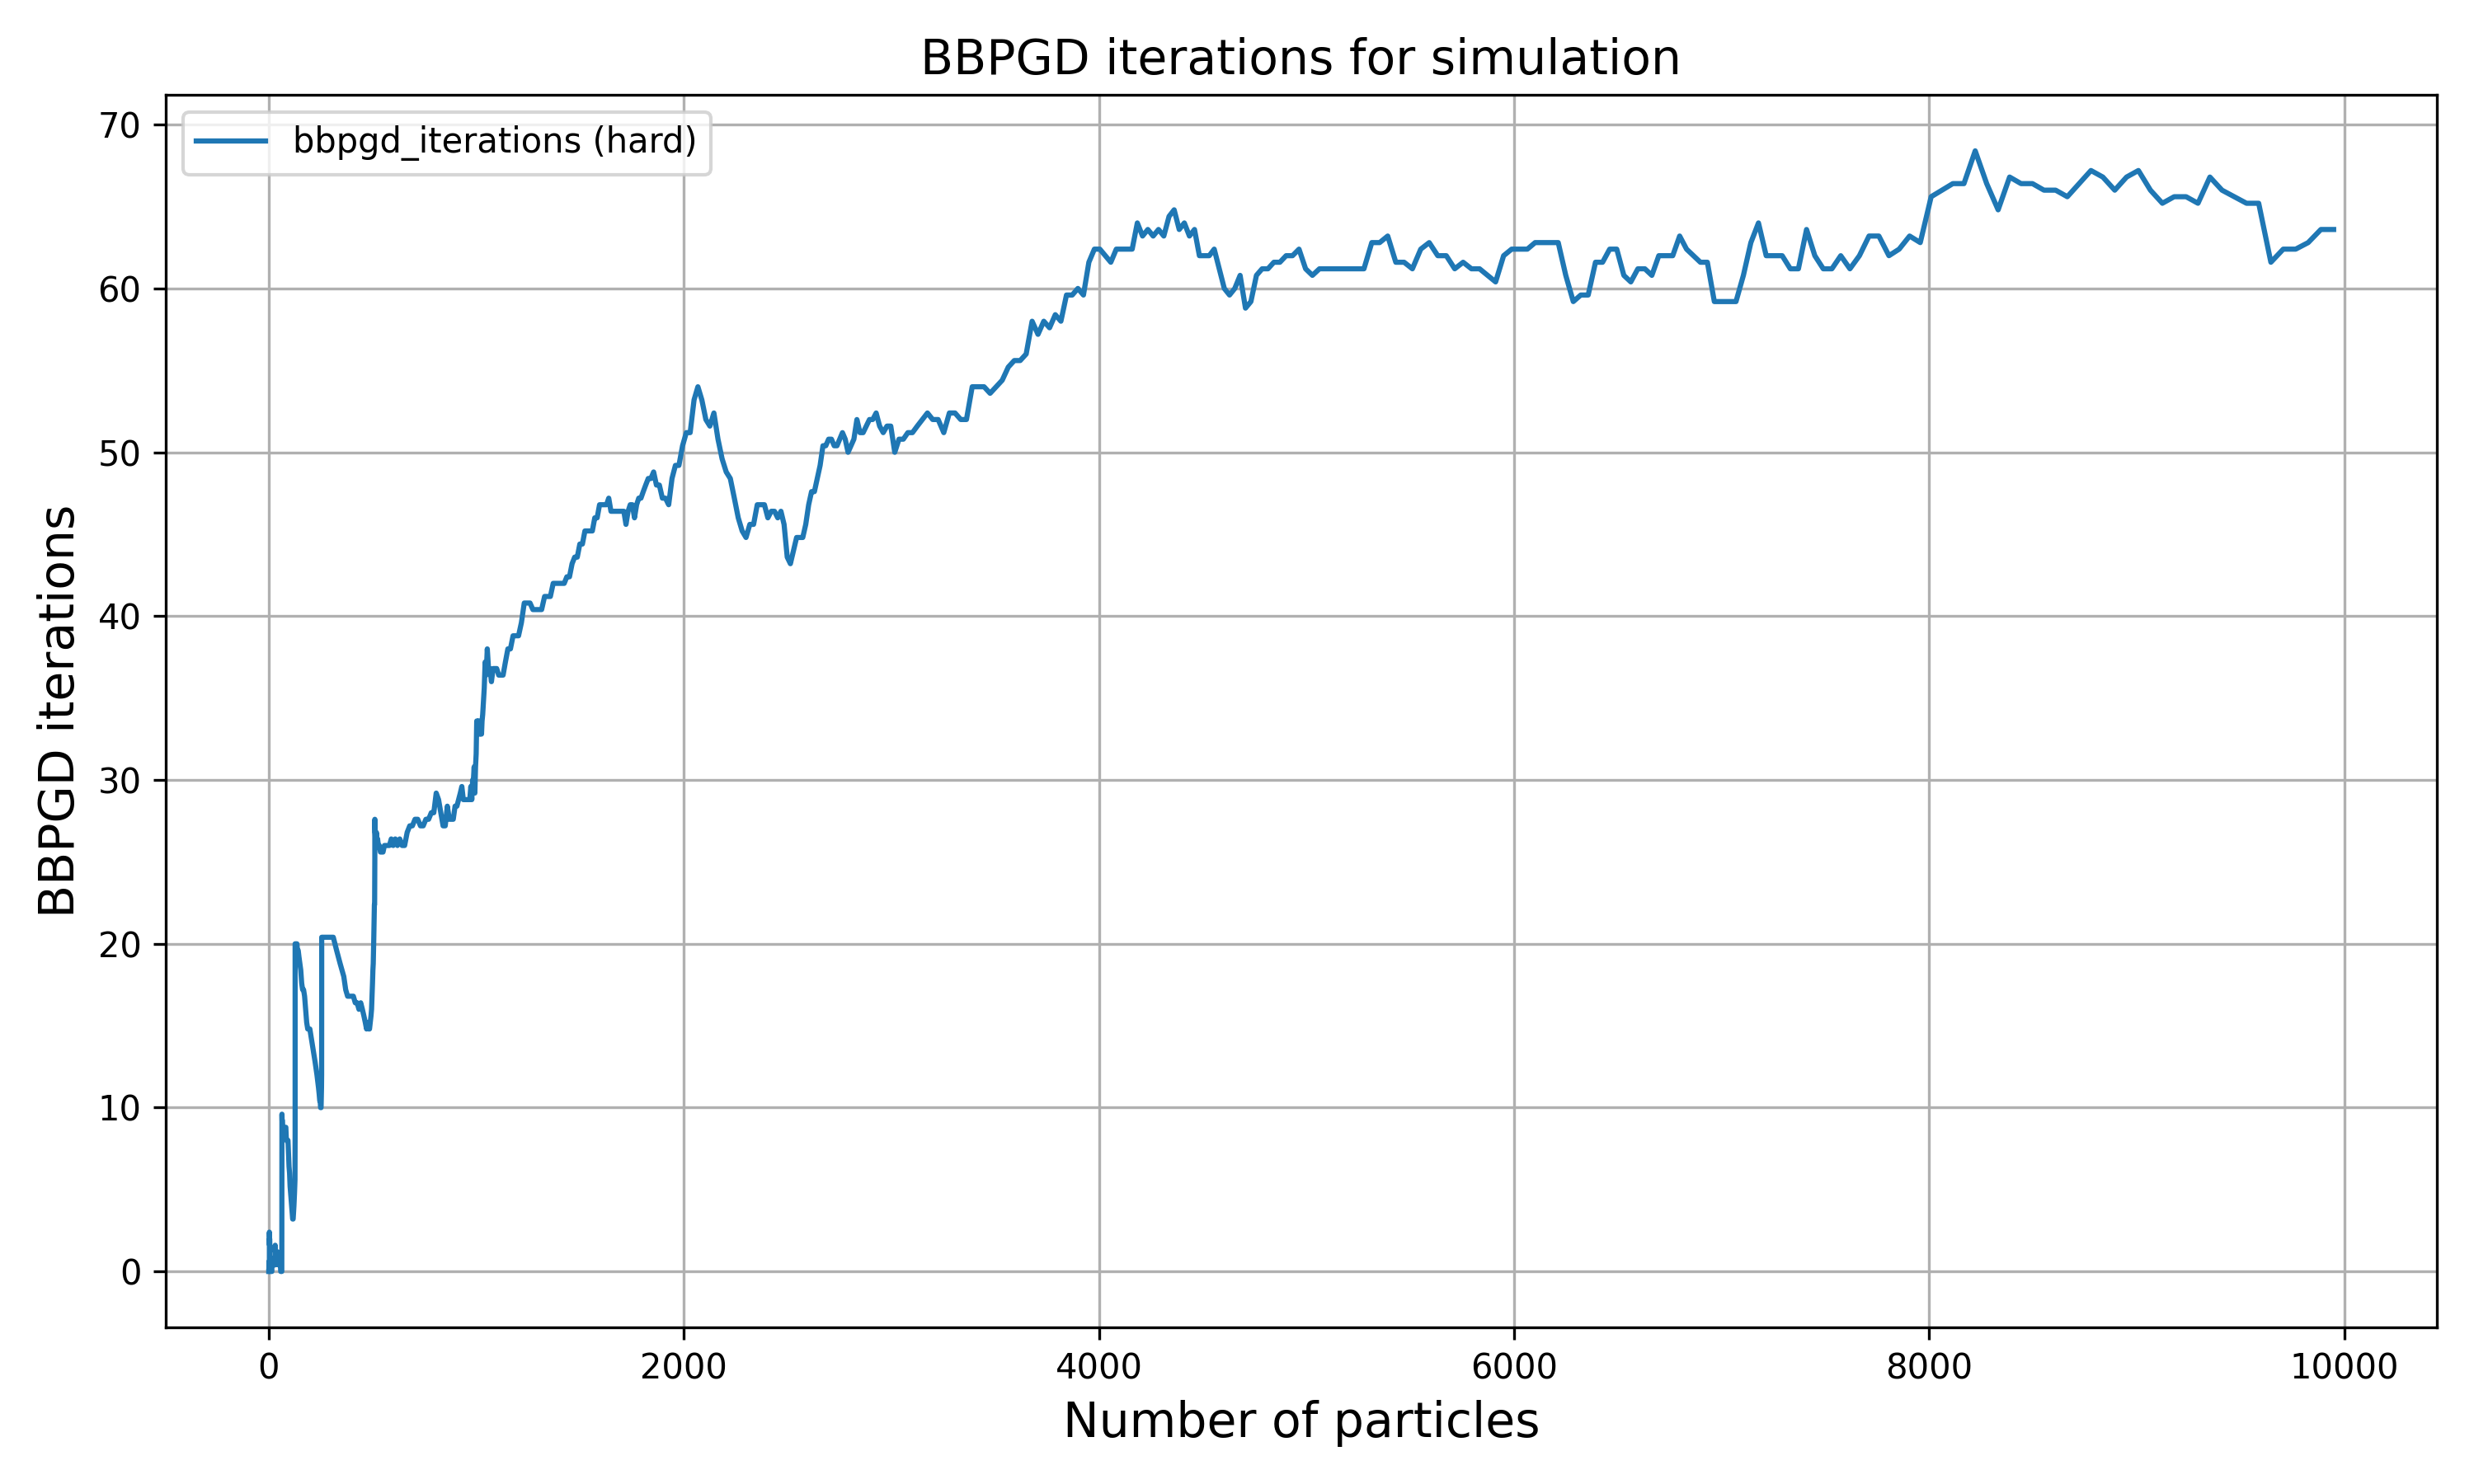
\includegraphics[width=\linewidth]{figures/comparisons/bbpgd_iterations_simulation.png}
    \caption{BBPGD iterations for the hard and soft collision models. To maintain constant particle separation, the hard model needs to solve an LCP iteratively at each time step. The required number of iterations increases with the number of particles.}
    \label{figure:bbpgd_iterations_simulation}
\end{figure}

\newpage
\section{Discussion}
\subsection{Model Selection Insights}


The choice between hard and soft collision models for simulating proliferating cell collectives presents a clear trade-off. The hard model offers precision in enforcing non-overlap but at a considerable computational cost due to LCP solving. The soft model, by employing continuous potentials, offers a potentially much faster simulation pathway, crucially important for exploring large-scale systems or parameter spaces. For many biological pattern formation scenarios, where the precise moment of contact is less critical than the emergent macroscopic behavior, the computational efficiency of the soft model makes it a highly attractive option.

\subsection{Biological Relevance}

Our findings suggest that the simplified mechanics of the soft collision model are sufficient to recapitulate key emergent behaviors like concentric ring formation. This implies that the fundamental drivers of these patterns may be robust to the specific details of collision resolution. The biological plausibility of the soft model lies in its ability to represent continuous pressure and proximity effects between cells, which might be more representative of cellular interactions than instantaneous, purely geometric constraints. The potential for faster simulations with the soft model could enable more extensive exploration of how proliferation rates, cell mechanics, and environmental factors influence colony morphogenesis.

\newpage

\section{Conclusion}

This work demonstrates that a computationally efficient soft collision model can effectively simulate proliferating cell collectives and reproduce complex emergent patterns observed in bacterial colonies, such as concentric rings. While the hard collision model provides exact non-overlap, its computational demands are substantial. The soft collision model offers a compelling alternative, promising significantly improved performance and scalability without a critical loss in qualitative pattern formation fidelity. This makes the soft approach a valuable tool for future large-scale simulations in computational biology and active matter research. Future work will focus on quantitatively detailing these performance benefits and exploring the soft model's behavior under more varied growth and environmental conditions.

\newpage
\tableofcontents


\bibliographystyle{IEEEtran}
\bibliography{literature}

\end{document}